\documentclass[conference]{IEEEtran}
\IEEEoverridecommandlockouts
\usepackage{cite}
\usepackage{amsmath,amssymb,amsfonts}
\usepackage{algorithmic}
\usepackage{graphicx}
\usepackage{textcomp}
\usepackage{color}
\usepackage{xcolor}
\usepackage{graphicx}
\usepackage{caption}
\usepackage{tabularx}
\def\BibTeX{{\rm B\kern-.05em{\sc i\kern-.025em b}\kern-.08em
    T\kern-.1667em\lower.7ex\hbox{E}\kern-.125emX}}
\begin{document}

\title{Ms. TROMM \\
- A Wise Secretary Always Thinking about You\\
}

\author{\IEEEauthorblockN{JIN HO KIM}
\IEEEauthorblockA{\textit{Dept. Information System} \\
\textit{Hanyang University}\\
Seoul, Korea \\
rlawlsgh1111@naver.com}
\and
\IEEEauthorblockN{EO JIN LEE}
\IEEEauthorblockA{\textit{Dept. Information System } \\
\textit{Hanyang University}\\
Seoul, Korea \\
djwls0317@gmail.com}
\and
\IEEEauthorblockN{GA HEE HAN}
\IEEEauthorblockA{\textit{Dept. Chinese Language and Literature} \\
\textit{Hanyang University}\\
Seoul, Korea \\
sarahan774@gmail.com}
\and
\IEEEauthorblockN{YU JIN HER}
\IEEEauthorblockA{\textit{Dept. Information System } \\
\textit{Hanyang University}\\
Seoul, Korea \\
roqhrcl777@hanyang.ac.kr}
}

\maketitle

\begin{abstract}
Abstract: LG provides LG ThinQ applications to connect its home appliances and consumers and provide consumers with a better experience. The application allows LG's refrigerator, kimchi refrigerator, wash tower, washing machine, dryer, air conditioner, water purifier, styler, air purifier, dishwasher, and oven control with smartphones. Among these many home appliances, we would like to take a deeper look at the link between ‘LG TROMM Styler’ and ‘LG ThinQ’. ‘LG TROMM Styler’ is a home appliance that has been steadily loved by many consumers since its launch because it relieves consumers' discomfort with clothes that are worn every day but cumbersome to manage. LG TROMM Styler provides indoor drying functions, including basic clothing management functions such as steam sterilization, deodorization, and wrinkle relief. This 'LG TROMM Styler' allows you to use functions such as energy monitoring and smartphone remote control when linked to the 'LG ThinQ' application. We would like to propose software that can be used in addition to these applications. This software recommends specific functions of the styler and allows it to operate remotely. Specifically, the software recommends appropriate clothing or styler functions by referring to weather information and calendar information on the user's smartphone. This is expected to help users in their daily lives because it allows users to prepare clothes that meet the weather and schedule in advance.
\end{abstract}

\begin{IEEEkeywords}
Mobile Application, Recommendation System, Artificial Intelligence, Styler, Clothing, Smart Secretary \\ \\
\end{IEEEkeywords}

\begin{table} [h]
    \centering
    \begin{tabular}{l|l|l}
    \hline
    \textit{\textbf{Roles}} & \textit{\textbf{Name}} & \textit{\textbf{Description}}
     & & & \\ \hline
    \textit{\textbf{User/Customer}} & \textit{EO JIN LEE} & \begin{tabular}[c]{@{}l@{}}User/Customer contemplates \\ what functions should be \\ added from the perspective \\ of users or customers. For \\ example, the 'LG TROMM \\ Styler' has a function of adding \\ scent to clothes in addition \\ to simply managing clothes neatly.\\ Consumers also have the need to \\ remotely use these specific \\ functions through the 'LG ThinQ' \\ application. In addition, the \\ application automatically identifies \\ the weather or my schedule and \\ plays a role in considering the \\ needs of the styler's clothing \\ management functions \\ appropriately. \end{tabular} \\ \hline
    
   \end{tabular}
\end{table}

\begin{table} [h]
    \centering
    \begin{tabular}{l|l|l}
    \hline
    \textit{\textbf{\begin{tabular}[c]{@{}l@{}}Product\\ Designer\end{tabular}}} & \textit{YU JIN HER} & \begin{tabular}[c]{@{}l@{}} A product designer is a person \\ with user-centered thinking \\ ability to sympathize with and \\ understand the user's experiences \\ and plays a role in creating \\ an overall framework for product \\ and services. It performs smooth \\ collaboration with other team \\ members with  excellent \\ communication skills. It focuses \\ on the usability of products \\ and services and performs \\ designs to provide better results.\end{tabular} \\ \hline
    \textit{\textbf{\begin{tabular}[c]{@{}l@{}}Software\\ Developer\end{tabular}}} & \textit{GA HEE HAN} & \begin{tabular}[c]{@{}l@{}} A software developer refers to \\ a person who makes software. \\ This includes discovering a \\ meaningful service and accurately \\ grasping the needs of a user who \\ wants to use the service. In \\ addition, there is a need for the \\ ability to design and code \\ these services and user needs \\ in software. Furthermore, the \\ software developer tests the \\ created program.  \end{tabular} \\ \hline
    \textit{\textbf{\begin{tabular}[c]{@{}l@{}}Development\\ Manager\end{tabular}}} & \textit{JIN HO KIM} & \begin{tabular}[c]{@{}l@{}} Development Manager manages \\ the overall part of the project, \\ such as the schedule/planning of \\ the project and the quality of \\ products and services. It also \\ manages/supervises the entire \\ software engineering process of \\ designing, developing, and testing \\ software from accurately grasping \\ user  requirements. In addition, \\ in this process, Development \\ Manager helps project participants \\ communicate smoothly.\end{tabular} \\ \hline
    \end{tabular}
    \renewcommand{\thetable}{\arabic{table}}
    \caption{Roles of Members}
    \label{table}
\end{table}    


\section{Introduction}
\subsection{Overall Introduction}
We are going to create this application with an emphasis on enhancing the value of LG TROMM Styler. Clothing functions as our second skin as one of the three basic elements of life, food, clothing, and shelter. We wear clothes every day and look at what the other person wears. In particular, it constitutes our egos through the process of choosing clothes and the habit of wearing clothes. Clothing is not only a basic purpose of protecting the body, but also a means of representing the value and status of the person wearing the clothes. Likewise, clothes are tools to complete humans, which are social animals.

However, it takes a lot of time and effort to manage the clothes to wear every day. Especially, in Korea, difficulties in managing clothing at home have increased due to air pollution such as fine dust. Due to this situation, the demand for clothing management devices at home increased, and in May 2011, LG launched the ‘LG TROMM Styler’ (hereinafter referred to as ‘Styler’). Styler is loved by allowing clothes to be managed at home for dry cleaning and shows high growth in sales rates. Furthermore, stylers are developing into comprehensive home appliances including indoor dehumidification functions as well as clothing management. 

In addition to this, LG increased device accessibility by linking its app called 'LG ThinQ' with a styler.‘ LG ThinQ’ is a representative home appliance management app that provides smart home services based on AI. With this application, you can control not only home appliances, but also all parts of the house, as well as check product status and malfunctions anytime, anywhere. In a situation in which the market environment is rapidly changing from 'supplier-centered' to 'consumer-centered, LG is providing these services, believing that the role of AI technology has grown.

However, we found that most users always worry in front of the Styler, "What should I wear tomorrow?" This is because they put clothes in the Styler to take full care of them for tomorrow schedule. In this situation, we have introduced an AI-based recommendation system(hereinafter referred to as ‘Ms.TROMM’) to Styler to reduce this time of concern and promote consumer-centered value. 

Ms.TROMM recommends modes that can be operated by the Styler, styling, and scent. First,  Ms.TROMM makes recommendations based on the user's calendar. By linking the calendar, Styler mode is recommended according to the user's schedule, and user can select the Styler operation by their preference. Second, Ms.TROMM uses the weather API to recommend suitable for the weather or a Styler mode that suits with weather. Third, Ms.TROMM identifies the clothes and the material of the clothes in the Styler and recommends the appropriate Styler mode and styling information for the clothes. Finally, data is accumulated through the process of receiving user feedback after all recommendations, and Ms.TROMM provides more sophisticated personalized recommendations. Through this, people can reduce their time of concern in front of the styler every evening or morning, and the need for a styler in our lives will also increase. Also, it is expected that users will be able to receive positive values for LG and styler if Ms.TROMM is installed in the ‘LG ThinQ’ application. We plan to create this application with an emphasis on increasing the satisfaction of styler users through Ms.TROMM, a system that allows users to use stylers and experience better.
\subsection{Problem Statement}\label{SCM}
\begin{itemize}
\item There is an application called ‘LG ThinQ’ as a mobile application that can be used in conjunction with LG home appliances. We thought that it would be better if a recommendation function was included in this application
\item It is very useful to use a styler to manage clothes, but since it takes a lot of time to manage clothes, there is a time constraint to take care of clothes to wear right away in the morning.
\item Therefore, we thought that the styler could be used more effectively if there was software that knew the user’s schedule and weather and sent a message to manage clothes in advance.
\item The software recommends clothes that users will like in the future based on feedback on past users’ tastes and recommendations. In other words, it helps you to use the styler efficiently by controlling the past and the future at once.\\
\end{itemize}

\section{REQUIREMENT}

\subsection{Entry}
If the user downloads and runs the application, the splash screen is required. The splash screen is a screen that appears for 1 to 2 seconds not to show the empty screen during loading of the app's data when running the application and will utilize the way to access the app screen naturally using the service's logo as the background. And if the user doesn’t have a login history on your phone, the onboarding page will be displayed to the user explaining why the main functions and functions of Ms. TROMM are useful. The onboarding page consists of a description of the overall application, the sign-up button and the login button.\\

\subsection{Login}
On the login page, a form screen appears where users can enter e-mails and passwords. Ms. TROMM authenticates whether you are a user registered in the DB with two elements: an e-mail and a password. At the bottom of the login button, there is a button to sign up for membership and go to the password change screen.\\
\begin{enumerate}
    \item Fail to Login: The re-input request pop-up has occurred.\\
    \item Sign up: Go to the member registration page.\\
    \item Find password: Go to the password search page.\\
    \item If the user log in for the first time: Go to Survey\\
    \item If the user has a log-in record: Go to Main Page\\
\end{enumerate}

\subsection{Sign up}
Ms. TROMM requires four types of information when signing up for membership. This is the email and password used to check DB registration and the gender and year of birth required to configure the initial recommendation. And there is a password verification field to reduce password-related errors. When the membership registration is completed, go to the login page. \\
\begin{enumerate}
    \item Invalid: If an invalid value is entered in each field, a remark requesting re-entry occurs under the field.\\
    \item Pass: If a valid value is entered in each field, a statement that it has been confirmed occurs under the field.\\
    \item Fail to Sign-up: If you do not fill out each field or press the membership button while entering an invalid value, a pop-up occurs that requires re-entry.\\
    \item Complete: A message congratulating membership and a button to go to the login page is exposed.\\
\end{enumerate}

\subsection{Survey}
When the user first logs in to Ms. TROMM, the survey page is exposed. The survey consists of contents that help set up the initial recommendation system. The survey consists of a total of three chapters (a style you usually wear often, a favorite color, and a favorite scent). Among them, the style you usually wear often offers different options depending on the gender value you entered when signing up for membership.\\
\begin{enumerate}
    \item Survey Guide Page: There is a brief description of the survey and a button to go to the survey page.\\
    \item Questionnaire page: It consists of a total of three chapters. Up to three options can be selected, and you can pass them without selecting them.\\
    \item If the user doesn't select an option: If you don't select it, a pop-up appears stating that the accuracy of the recommendation may decrease.\\
    \item Warning: When clicking on the bottom nav during the survey, a pop-up will occur indicating that the user cannot go to another page.\\
    \item Complete: When the user complete the survey, press the button on the exposed screen to go to the main page.\\
\end{enumerate}

\subsection{Main Page}
Users can check the functions in the app at once on the main page. \\
\begin{enumerate}
    \item Date and weather widget: The user can check today's date and weather.\\
    \item Today's recommendation widget: The user can check today's recommendation.\\
    \item Styler Control Widget: Styler Control Possible\\
    \item Current my house widget: The user can check the temperature and humidity of your house.\\
\end{enumerate}

\subsection{Pop-up notification}
Recommendations and styler-related information from Ms. TROMM are displayed through pop-ups.\\
\begin{enumerate}
    \item Today's Recommendation Pop-up: consists of buttons that receive content and user responses.\\
    \item Control Recommendation Pop-up: consists of content and confirmation buttons.\\
    \item General pop-up: consists of content and confirmation buttons.\\
\end{enumerate}

\subsection{Notification}
It is a menu in which all pop-ups are displayed within Ms. TROMM. Everything the user has seen is recorded.\\

\subsection{Recommendation}
It is a menu where recommendations are exposed. In this menu, users can check two tabs: today's recommendation based on schedule and weather, and control recommendation using clothing information in the styler. When the user first enters the recommendation menu, a page with a description of each element in the recommendation menu is exposed. If the user wants to see the recommendation and run the fragrance control system inside the styler, the user can click on the fragrance recommendation list to run it.\\
\begin{enumerate}
    \item Menu description screen: Exposed when entering for the first time.\\
    \item Move the recommended menu: Check and move the two recommended tabs with the menu button at the top.\\
    \item  Apply Scent: You can apply the recommended scent within the styler with a pop-up that appears by pressing the Scent button.\\
\end{enumerate}

\subsection{My Closet}
My closet is a menu that can be accessed anywhere in Ms. TROMM with floating action buttons. You can see the registered clothes in my closet, and you can check the information you entered when registering clothes. And each outfit tells you how many stylers you need in a comment.\\
\begin{enumerate}
    \item Information Check: The information you wrote when you registered your clothes, the registration date of your clothes, and the date you last put your clothes in the styler are exposed.\\
    \item Register new clothes: Ms. You can register new clothes in TROMM DB. This information is linked to a smart mirror. When registering new clothes, a form screen appears to enter the information on the clothes.\\
\end{enumerate}

\subsection{Styler}
This menu is linked to the styler so that the user can control the styler in this app. It provides a button to operate all the operating functions in the styler. The button placement was adjusted by referring to another remote control application.\\
\begin{enumerate}
    \item Styler on/off\\
    \item Choose a styler course\\
\end{enumerate}

\subsection{All}
This is a menu that allows users to check the basic application information. You can check the application version information in this menu. In addition, you need a function that allows users to check and modify what they wrote when signing up. And you can check the terms and conditions of personal information used within the application.\\

\section{DEVELOPMENT ENVIRONMENT }
\subsection{Choice of software development platform}
Our main development environment is Windows and MacOS. In the case of Windows, terminals that can be used even in windows such as Powershell were used to create a linux environment, and in the case of MacOS, built-in linux environment and terminals were used. Ms.TROMM in order for consumers to receive recommendations faster and immediately control devices such as stylers and smart mirror. Ms.TROMM was manufactured based on mobile applications. In addition, Ms.TROMM so that more users can use it in various mobile operating systems. The frontend framework of Ms.TROMM selected 'Flutter', a representative cross-platform framework. Currently, Google's Android accounts for the majority of global mobile platforms, and Apple's iPhone accounts for about 15\%, but Apple's iPhone users' consumption patterns and loyalty to electronics are quite different from Android users, and iPad, which accounts for a large portion of the tablet market, so the actual usage rate is very high. In fact, looking at the mobile operating system market share, including the tablet market, it can be seen that the proportion of iOS (including iPadOS) has increased by about 30\%. Therefore, we have adopted Flutter, a mobile/web/desktop cross-platform framework launched by Google based on the Dart Programming language, as a frontend framework, satisfying all of these demands and further considering future desktop applications. In the case of backend server, Python-based Flask, which implements artificial intelligence-based services and has well-established statistical and analysis packages, was adopted. Flask has the advantage of being easy to create API servers and very light. In addition, since Flask has a high degree of freedom, such as being able to change and respond immediately according to the purpose of development when there is not much time left, It was adopted because it was considered the most suitable web framework for Ms.TROMM development.\\ \\ 

\begin{figure}[]
\centerline{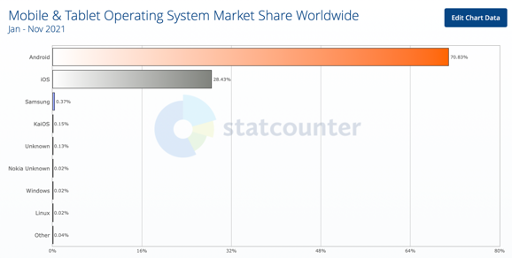
\includegraphics{assets/그림1.png}}
\caption{Mobile \& Tablet OS Market Share Rate}
\label{fig}
\end{figure}

\begin{figure}[]
\centerline{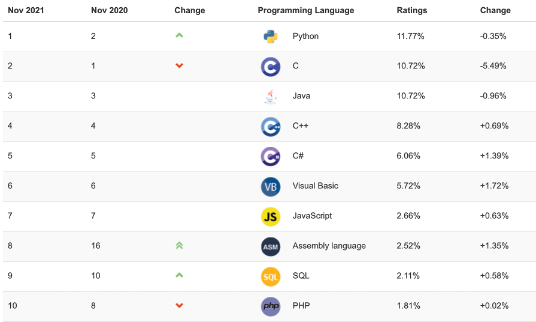
\includegraphics{assets/그림12png.png}}
\caption{TIOBE INDEX}
\label{fig}
\end{figure}


\begin{table}[ht]
    \centering
    \begin{tabularx}{\columnwidth}{X|X}
    \hline
    \textit{\textbf{Name}} & \textit{\textbf{Development Environment}}
     & & \\ \hline
    \textit{\textbf{JIN HO KIM}} & MacOS, Python 3.8.5    
     & & \\ \hline
    \textit{\textbf{EO JIN LEE}} & Windows, Python 3.9.0
     & & \\ \hline
    \textit{\textbf{GA HEE HAN}} & Windows, Python 3.9.2
     & & \\ \hline
    \textit{\textbf{YU JIN HER}} & Windows, Python 3.7.1
     & & \\ \hline
    \end{tabularx}
    \renewcommand{\thetable}{\arabic{table}}
    \caption{Develop Environment}
    \label{tab:table}
\end{table}
\break

\begin{table}[h]
    \centering
    \begin{tabular}{c|l}
    \hline
    \multicolumn{1}{l|}{\textit{\textbf{Tools and Language}}} & \textit{\textbf{Reason}} 
     & & \\ \hline
    \textit{\textbf{Python}} & \begin{tabular}[c]{@{}l@{}} Python is one of the programming languages \\ that many people love around the world. \\ TIOBE announces the rankings of world-\\famous programming languages every month,\\ representing them as "TIOBE INDEX,"\\ and Python was ranked No. 1 programming \\ language loved by people around the world as \\ of November 2021. Python is also the base \\ language for Flask, a web server framework, \\ but it provides excellent modules related \\ to artificial intelligence. In addition, it provides \\ a Pandas, Numpy module, etc. necessary for \\ data analysis and processing of collected data. \end{tabular} \\ \hline
    \textit{\textbf{MySQL}} & \begin{tabular}[c]{@{}l@{}} We need a database that stores data from users \\ who signed up for membership to use the \\ Ms.TROMM service, stores schedule data \\ used for recommendations, and responses from \\ users, and provides better service \\ recommendations based on this. Therefore, \\ we intend to manage the basic database \\ using MySQL. \end{tabular} \\ \hline
    \textit{\textbf{Flutter(Dart)}} & \begin{tabular}[c]{@{}l@{}} Flutter is a Dart language-based cross-platform \\ framework launched by Google. So, \\ Ms.TROMM was developed based on Flutter \\ so that it could be expanded to web and \\ desktop apps in the future. In addition, \\ even though it is a cross-platform, it provides \\ native-class performance and various extensions, \\ makes it easy to check the UI in a simple \\ virtual environment, and supports plug-ins \\ from famous IDE and code editors, so Flutter \\ was selected as the frontend framework. \end{tabular} \\ \hline
    \end{tabular}
    \renewcommand{\thetable}{\arabic{table}}
    \captionsetup{justification=centering}
    \caption{Tools and Programming Languages \\ used for development}
    \label{tab:table}
\end{table}


\begin{figure}[htbp]
\centerline{
\includegraphics{assets/flutter.png}}
\caption{Cross-platfrom framework 'Flutter'}
\label{fig}
\end{figure}
\break

\subsection{Cost estimation}
To implement Ms.TROMM, it was necessary to obtain data from the database or to obtain real-time information from the server while communicating with the server in real-time. Therefore, real-time servers were hosted or several APIs were needed. However, in the process of development, we tried to develop open APIs, free modules, and free servers first. Therefore, the server also implemented a real-time server through the Heroku service, which is a server that provides free hosting up to certain traffic. In addition, the process of bringing up weather and calendar information used open APIs that were released free of charge to Google and others. However, JetBrain's Datagrip was used in the process of controlling data, and this application is provided free of charge only to students. Later, Ms.If the TROMM service is expanded, traffic on the server may increase and various copyright problems may occur, so it would be desirable to use paid services when expanding the service. \\ \\ \\ \\ \\

\subsection{Software in use}
\begin{enumerate}
    \item LG ThinQ, LG SmartHome Application\\
    \centerline{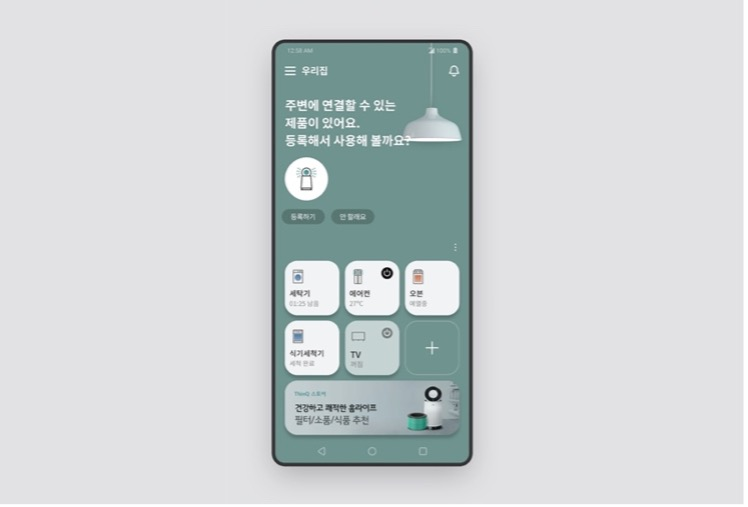
\includegraphics[scale=0.30]{assets/thinkq.jpg}}

        LG Electronics uses the 'LG ThinQ', an application to control its smart home appliances. In addition, in the case of smart mirror, it can be controlled through the 'LG Smart Home' as a key home appliance for the smart home ecosystem that will be built as soon as possible. Through these two apps, LG Electronics will bridge users and smart devices so that users can monitor and control their homes anytime, anywhere. Our application is also an app to build a better ecosystem between users and smart devices. Our app is a smart assistant-like application that integrates the environment in which users use smart devices, checks minor things in advance that users may miss, and recommends the best way. \\ \\
    \\ 
    \item VSCode(Visual Studio Code) \\ \\
    \centerline{
\includegraphics{assets/vs.png}}
    VSCode is an open source-based text editor published by Microsoft. VSCode is a text editor, not an IDE, but has the advantage of being able to install various expansion packs. In addition, it has its own terminal function. Supporting various languages, The development environment for data and artificial intelligence technologies used by Ms.TROMM is excellent. In addition, VSCode was adopted as a text editor because of its excellent interworking with Git, a version control system.\\ \\ \\ \\ 
    \item GitHub\\\\
    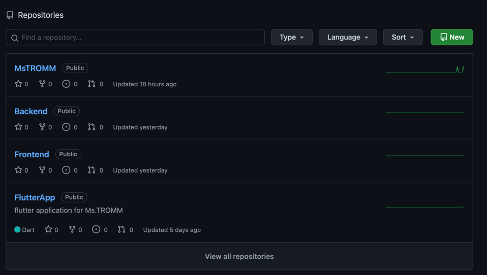
\includegraphics[scale=0.9]{assets/Gtib.png}
    \\ \\ GitHub serves as a repository for Git, a distributed version control system. During development, several people go through a collaborative process of adding and deleting various functions, which can lead to confusion in this process without a version control system. Github is a web-based service that allows you to intuitively understand the team members' version control process. In addition, simple processes such as simply uploading and downloading files can be easily controlled using GUI tools such as Github Desktop. \\
    
    \break
    
    \item Android Studio \\ 
    \centerline{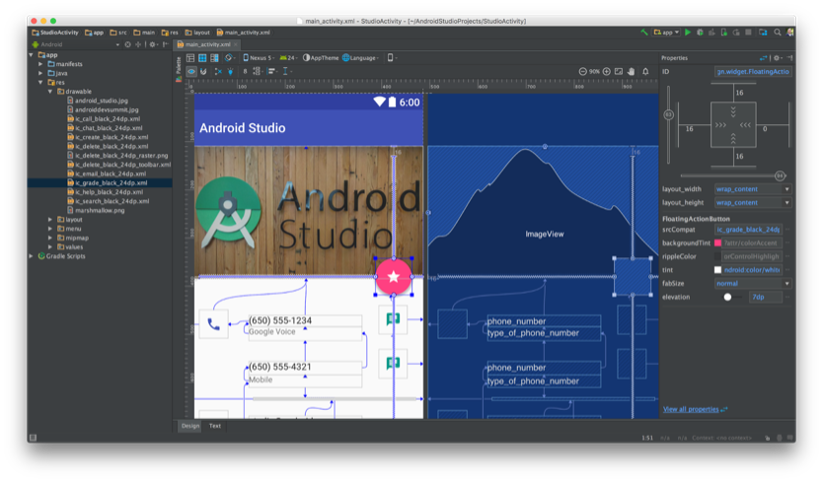
\includegraphics[scale=0.9]{assets/as.png}}
    In the case of Ms.TROMM, since it is basically a mobile app, an integrated development environment (IDE) for mobile apps was needed, and Android Studio, which team members were relatively familiar with, was adopted as IDE. Both Flutter and Android Studio, which we adopted as the Frontend Framework, are platforms announced by Google, so they are highly interconnected, so there was no big problem in developing them. The advantage of being able to develop while checking the progress of the app through the UI is also the reason for adopting Android Studio. \\\\\\\\\\\\
    
    \item Heroku\\\\
    
\includegraphics{assets/Heroku.png}
    \\ \\ Heroku is a service that allows free hosting of websites through git. It is a cloud platform as a service (PaaS) that supports multiple programming languages. In general, when developing or implementing an app, it provides a platform that enables applications to be developed, executed, and managed without the complexity of creating and maintaining related infrastructure. \\
    
    \break
    
    \item Firebase\\\\
    
\includegraphics[scale=0.7]{assets/firebase.png}
    \\ \\ Firebase is a backend as a service (BaaS) that provides the necessary functions for web and mobile development. In other words, it is a service that helps you focus on front-end development without designing or implementing servers separately through back-end development. Features include real-time databases, easy user authentication, cloud storage, hosting, app testing, and profit generation. \\
    
    \item DBdiagram \\ \\
    \centerline{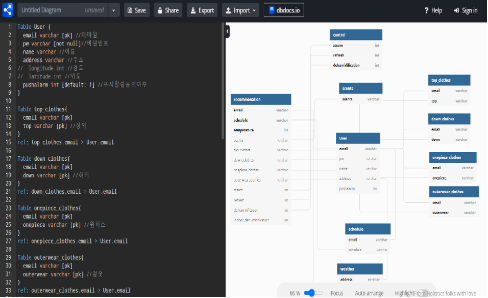
\includegraphics[scale=0.9]{assets/DB.png}}
    \\ It is a free, simple tool to draw ER diagrams by just writing code. So, the user can draw entity-relationship diagrams, painlessly. ERD is a very important development product because it can be used to see the model at a glance when implementing functions. Using this site, ERD can be configured through a code similar to SQL. If related codes such as tables and indexes are inserted without drawing ERD separately, ERD is automatically generated. It is also very useful because it can be modified based on code even when modifying.\\ \\

    \item MySQL \\ \\
    \centerline{
\includegraphics[scale=0.1]{assets/MySQL.png}}
    \\ MySQL is the most widely used open-source database worldwide. It is an open-source relational database management system (RDBMS) that uses the standard database query language SQL (Structured Query Language) and features very fast, flexible, and easy to use. It supports multi-user, multi-threads, and provides an application interface (API) for C, C++, Eiffel, Java, Pearl, PHP, Python scripts, and the like. It can be used in Unix, Linux, and Windows operating systems. The Linux operating system, Apache server program, MySQL, and PHP script language composition are free programs that are developed as open-source despite good interworking, so MySQL was also adopted in the development of Ms. TROMM.\\ \\ 
    
    \item SQLAlchemy \\ \\
    \centerline{
\includegraphics[scale=0.1]{assets/sqlalchemy.jpg}}
    \\ SQLAlchemy is an open-source SQL toolkit and object-relational mapper (ORM) for the Python programming language. The advantage is that it is possible to focus on business logic with object-oriented code. It also increases reuse and maintenance convenience and reduces dependence on DBMS. Because of these advantages, we decided to use SQLAlchemy with Ms. TROMM's recommendation system.\\ \\ \\ \\ 
    
    \item Datagrip \\ \\
    \centerline{
\includegraphics[scale=0.5]{assets/datagrip.png}}
    \\ A DBA tool which is aimed at developers who work with SQL databases. In other words, it is a GUI development tool that facilitates DB development and management. A lite version of DataGrip is embedded within the Ultimate edition of some of JetBrains' IDEs.\\ \\ \\ \\ 
    
    \break
    
    \item flask\\ \\
    \centerline{
\includegraphics[scale=0.5]{assets/flask.png}}
    Flask is a micro web framework written in Python. It is classified as a microframework because it does not require particular tools or libraries. It has no database abstraction layer, form validation, or any other components where pre-existing third-party libraries provide common functions. However, Flask supports extensions that can add application features as if they were implemented in Flask itself. Extensions exist for object-relational mappers, form validation, upload handling, various open authentication technologies and several common framework related tools. \\ \\ \\ \\ \\ \\ \\ \\
    
    \item numpy \\ \\
    \centerline{
\includegraphics[scale=0.5]{assets/numpy.png}}
    NumPy is a library for the Python programming language, adding support for large, multi-dimensional arrays and matrices, along with a large collection of high-level mathematical functions to operate on these arrays.The ancestor of NumPy, Numeric, was originally created by Jim Hugunin with contributions from several other developers. In 2005, Travis Oliphant created NumPy by incorporating features of the competing Numarray into Numeric, with extensive modifications. NumPy is open-source software and has many contributors. NumPy is a NumFOCUS fiscally sponsored project. \\ \\
    
    \break
    
    \item pandas \\ \\
    \centerline{
\includegraphics[scale=0.2]{assets/pandas.PNG}}
    Pandas is a software library for analyzing and manipulating data written in Python language. Pandas provide data for manipulating and operating numerical tables and time-series data, which can be used free of charge under Article 3 BSD license conditions. Pandas is named after the first letter of "PANel DATA," a term used in econometrics. Pandas use a structure called DataFrame modeled after the data. Frame structure used in R, many of the functions used in data. The frame of R can be used without difficulty. Moreover, because Python operates on a language-based basis with good accessibility, it has become an essential library for those who enter Python for data analysis. \\ \\ \\ \\ \\ \\ \\ \\ \\ \\ \\
    
    \item Marshmallow \\ \\
    \centerline{
\includegraphics [scale=0.3] {assets/marshmallow.png}}
    Marshmallow is an ORM/ODM/framework-agnostic library for converting complex datatypes, such as objects, to and from native Python datatypes. Marshmallow schemas can be used to validate input data. And it can be used to deserialize input data to app-level objects. Also it can be used to serialize app-level objects to primitive Python types. The serialized objects can then be rendered to standard formats such as JSON for use in an HTTP API \\ \\
    
    \item Swagger \\ 
    \centerline{
\includegraphics{assets/Swagger.png}}
    Swagger is a framework for Open API Specification (OAS). Swagger is used together with a set of open-source software tools to design, build, document, and use RESTful web services. Swagger includes automated documentation, code generation (into many programming languages), and test-case generation. Simply put, Swagger is an API Spec document. The method of managing APIs through Excel or guide documents requires periodic updates, so it is not easy to manage and takes a long time. So, we can easily manage and test API documents by automating API Spec documents using Swagger. \\ \\   

    \item XCode \\ 
    \centerline{
\includegraphics[scale=0.3]{assets/xcode.png}}
    Xcode consists of a suite of tools that developers use to build apps for Apple platforms. Use Xcode to manage your entire development workflow — from creating your app to testing, optimizing, and submitting it to the App Store.\\ \\ \\ \\
    
    \item Google API \\ 
    \centerline{
\includegraphics[scale=0.3]{assets/googleapi.jpg}}
    API is an application programming interface that allows users to exchange requests and responses from different programs such as clients and servers. API allows products/services to communicate with each other without knowing how to implement them and saves time and money by simplifying the application development process. It is divided into an open API and a private API according to the method and purpose of use. Open APIs can be easily accessed and shared by anyone, and private APIs provide information only to some authorized users. (Google API is an open API.) \\ \\ 
    
    \item Adobe XD \\ \\
    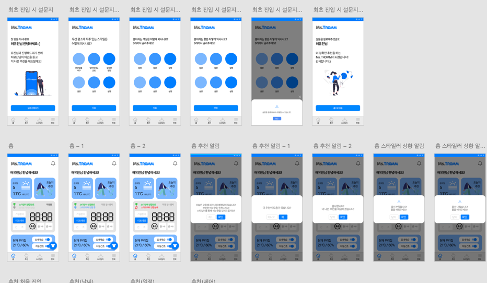
\includegraphics[scale=0.9]{assets/XD.png}
     \\ \\Adobe XD is an application for prototyping PCs, mobile Internet pages, and mobile apps released by Adobe. Since Ms.TROMM is a mobile app-based service, it was necessary to think about how users could feel the best experience when providing the app. Therefore, it is possible to intuitively prototype the operation of an Internet page or app operating in a corresponding environment through Adobe XD. In addition, the app development can be made easier by linking the prototype made in this way with Zeplin.\\ \\ \\ \\
    
    \item Zeplin\\ \\
    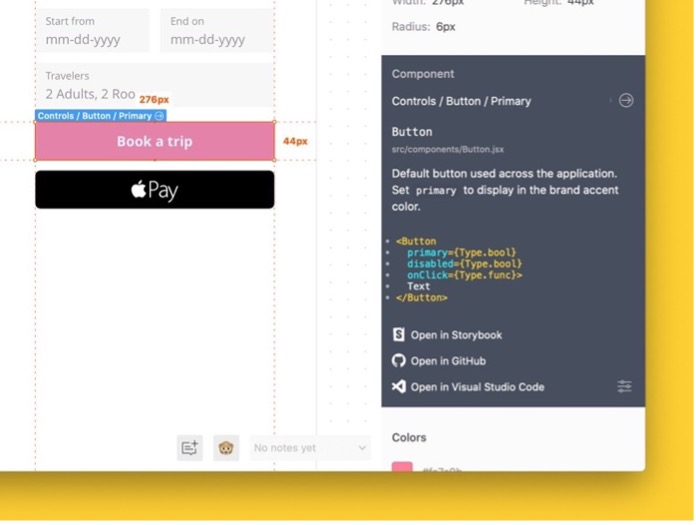
\includegraphics[scale=0.32]{assets/Zp.jpg}
    Zeplin is a software that helps designers and developers collaborate, and through Zeplin, you can convert design elements into development information (e.g., font, size, size, etc.). While developing apps through Zeplin, you can solve problems that may not be faithful to functional implementation while calculating design elements too deeply. 
    
\end{enumerate}{}

\subsection{Task distribution} 
\begin{table} [h]
    \centering
    \begin{tabular}{l|l|l}
    \hline
    \textit{\textbf{Tasks}} & \textit{\textbf{Name}} & \textit{\textbf{Description}}
     & & & \\ \hline
    \textit{\textbf{\begin{tabular}[c]{@{}l@{}}Frontend\\ Developer\end{tabular}}} & \textit{GA HEE HAN} & \begin{tabular}[c]{@{}l@{}} The front-end development job performs \\ work on business logic configuration and \\ user interface through the output and \\ input of data from the backend application \\ programming interface (API). In short, \\ it can be said that it is the job of \\ developing everything the user sees with \\ his or her eyes. It is the first impression \\ of Ms. TROMM  because it is the first part \\ that the user searches for service \\ information and sees when using it.\\ The fact that it serves as an intermediate \\ bridge between the backend and \\ the planning is also a feature that\\ distinguishes other jobs from frontend \\ development. \end{tabular} \\ \hline
    \textit{\textbf{\begin{tabular}[c]{@{}l@{}}Backend\\ Developer\end{tabular}}} & \textit{\textbf{\begin{tabular}[c]{@{}l@{}}EO JIN LEE\\ JIN HO KIM\end{tabular}}} & \begin{tabular}[c]{@{}l@{}} Backend development implements the overall \\ logic of all services, including cloud and \\ hosting, provided by Ms. TROMM. \\ Backend developers develop APIs to respond \\ to requests from clients on API servers. \\ In addition, backend developers will design \\ a table (space) that can conceptually separate \\ data in the application for database \\ management. Finally, we use the cloud to \\ build servers.  \end{tabular} \\ \hline
    \textit{\textbf{\begin{tabular}[c]{@{}l@{}}Product\\ Designer\end{tabular}}} & \textit{YU JIN HER} & \begin{tabular}[c]{@{}l@{}} The product designer conceives what functions \\ are needed and how to implement them based \\ on the requirements for Ms. TROMM.\\ To analyze requirements, product designer\\ benchmarks users, designs, services \\ comprehensively and derives insights. \\ Based on Insight, find appropriate ways \\ to meet the requirements, establish service \\ policies and processes, and design screens. \end{tabular} \\ \hline
    \end{tabular}
    \renewcommand{\thetable}{\arabic{table}}
    \caption{Task distribution of Members}
    \label{table}
\end{table}    

\section{SPECIFICATION}
    \begin{figure}[htbp]
\centerline{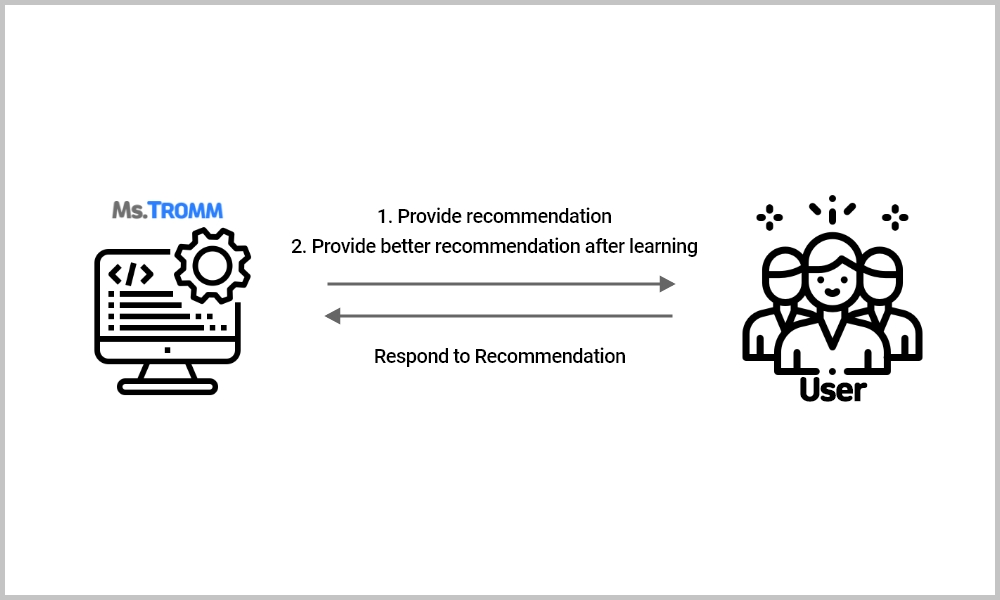
\includegraphics[scale=0.2]{assets/Whole application.jpg}}
\label{fig}
\end{figure}
This picture shows our whole application. Ms. TROMM's recommendation system provides recommendations to users. At this time, the user's reaction is recorded in the DB, and the recommendation system proceeds with learning based on this reaction. And when the next recommendation situation comes, the recommendation system provides recommendations to users again. \\ \\ \\ \\ 

\subsection {Entry} \\
\begin{enumerate}
    \item Splash screen \\ \\
     \centerline{
\includegraphics[scale=0.32]{assets/스플래쉬 화면.jpg}}
    \begin{itemize}
    \item[] This is the start page when you run the app. It is exposed for 1 to 2 seconds not to show an empty page during the app's data loading time.
    \end{itemize}
    
    \break
    
    \item Onboarding screen \\ \\
    \centerline{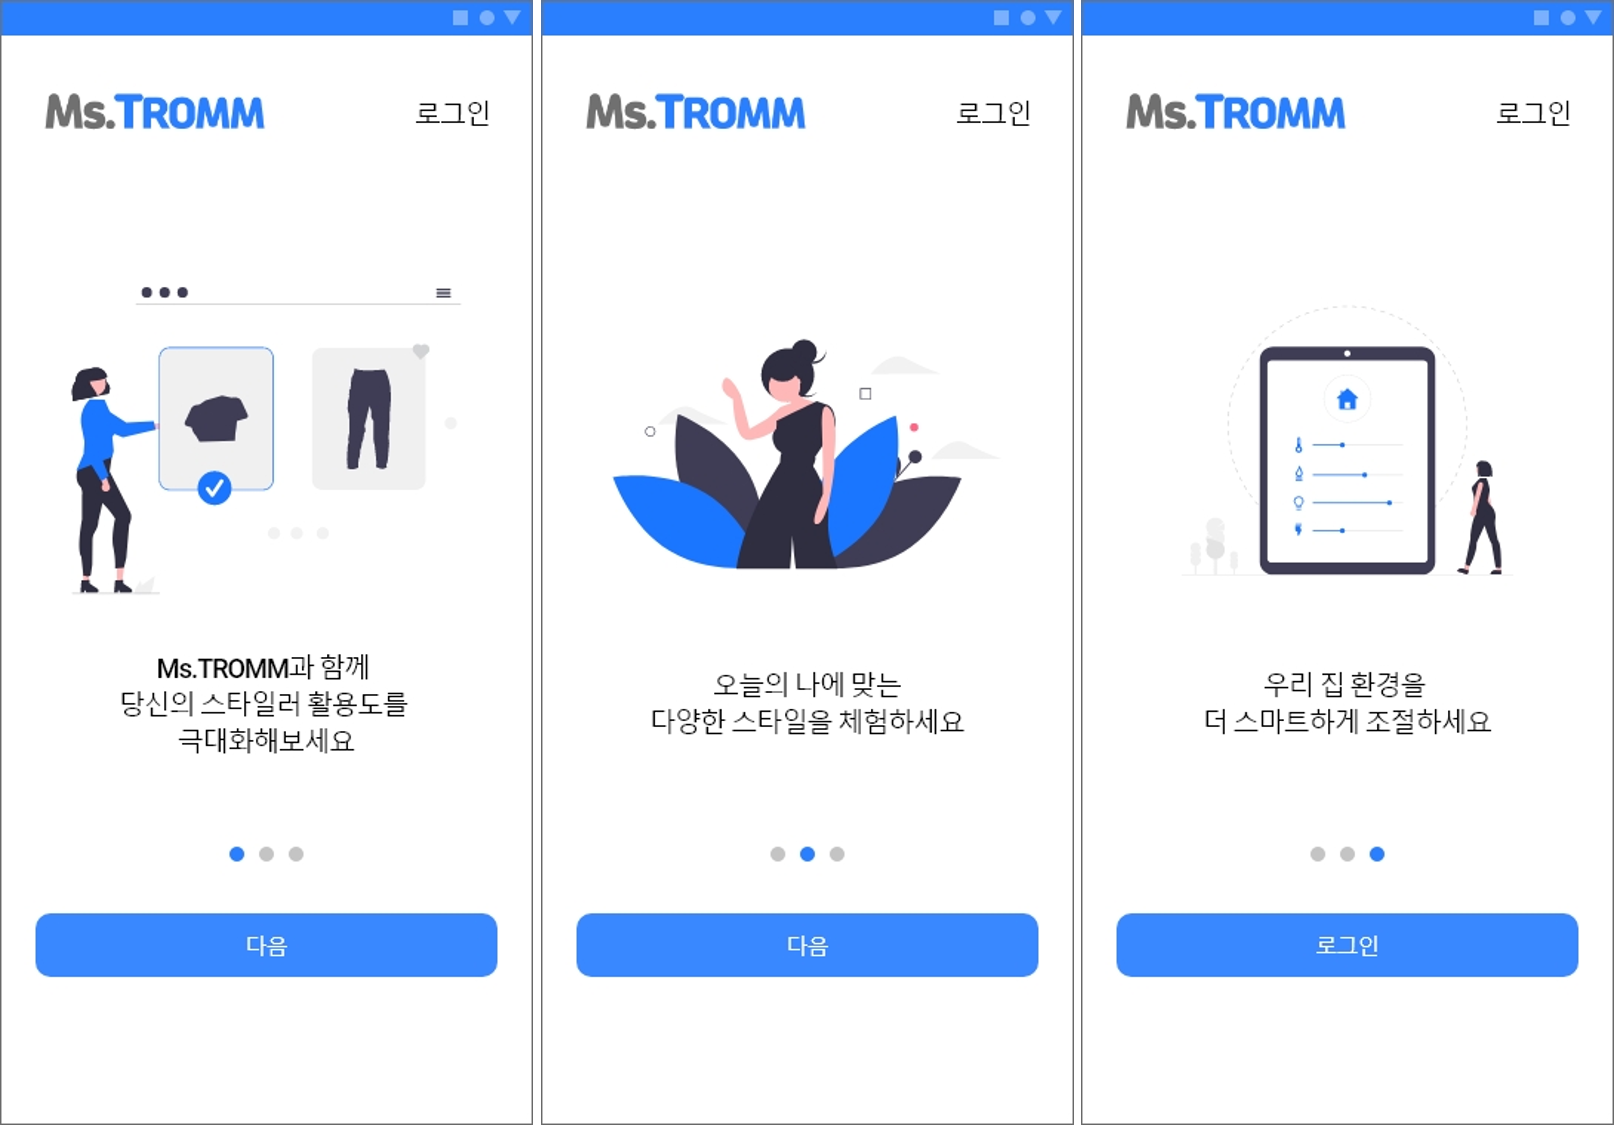
\includegraphics[scale=0.25]{assets/온보딩.png}}
    \begin{itemize}
    \item[] It is a page that prevents the deletion of apps by clearly showing users the reason for the existence of apps. It consists of a total of three pages explaining why Ms.TROMM's main functions and functions are useful.\\ \\ \\
    \end{itemize}
    \item Onboarding Button \\ \\
    {
\includegraphics[scale=0.75]{assets/온보딩_다음.jpg}}
    \begin{itemize}
    \item[] Put the next button at the bottom of the page so that you can move on to the next page.
    \end{itemize}
    {
\includegraphics[scale=0.75]{assets/온보딩_로그인.jpg}}
    \begin{itemize}
    \item[] And on the third page, it changes to the login button to the next button location as shown in the picture. 
    \\ If you have login data on your phone, do not expose the onboarding page. When the splash screen is terminated, the login page is immediately exposed.
    \end{itemize}
    \end{enumerate}
    \break

\subsection {Login} 
Ms.TROMM receives two types of information (email, password) for login.\\
\begin{enumerate}
    \item Login form screen \\ \\
    \centerline{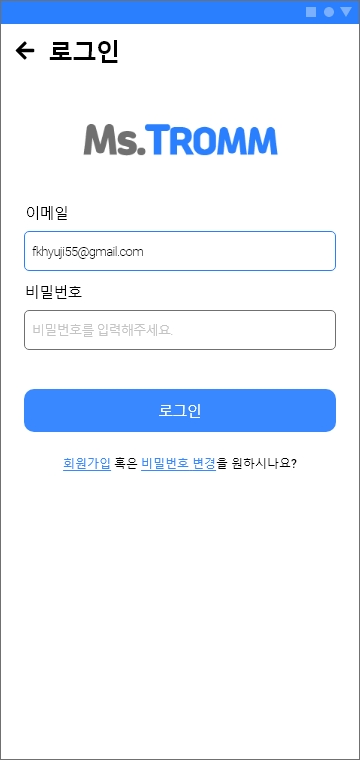
\includegraphics[scale=0.32]{assets/로그인1.jpg}}
    \begin{itemize}
    \item[] A login form screen appears where you can enter your email and password. The login button is exposed at the bottom of the field, and there are buttons below the button to sign up for membership and go to the password change page. \\
    \end{itemize}
    \item Login failed screen \\\\
    \centerline{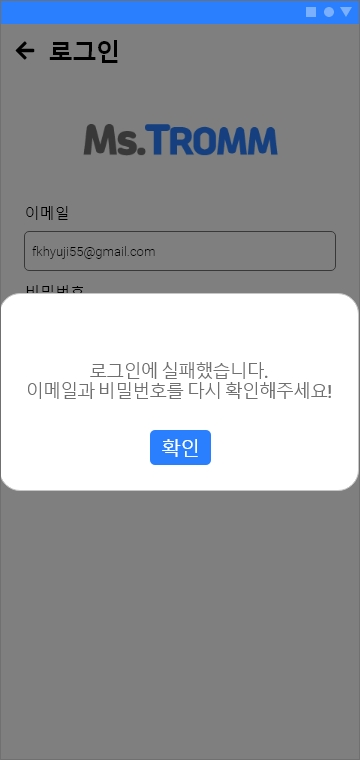
\includegraphics[scale=0.32]{assets/로그인2.jpg}}
    \begin{itemize}
    \item[] If login information that is not in the DB is entered, login failed and a pop-up with 'Please check your email and password again!' comment is displayed at the bottom. When you click the gray area or 'x button' or 'OK button', the pop-up will end and the previous one will be exposed again. \\ \\
    \end{itemize}
    \item Changing the password \\ \\ \\
    \centerline{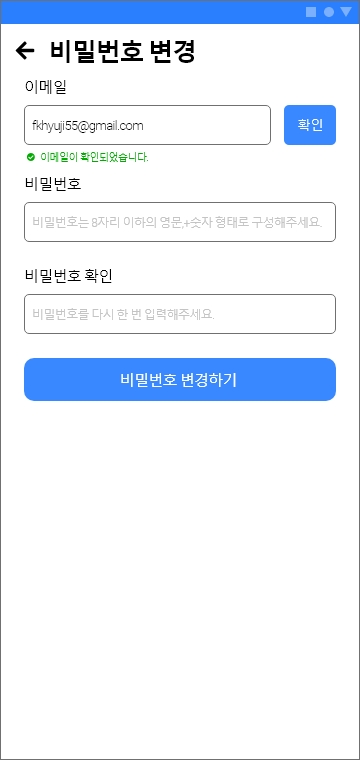
\includegraphics[scale=0.32]{assets/비밀번호 변경.jpg}}
    \begin{itemize}
    \item[] It is a page that supports password change when a user forgets his or her password. In the case of e-mail input, there is an e-mail confirmation field to verify that it is currently in DB. Hereinafter, there is a field where a new password can be set, and there is a password confirmation field to prevent password errors. \\ \\ 
    \end{itemize}
    \end{enumerate}
    
\subsection{Sign up}
This is the membership form page. Ms.TROMM receives three types of information (name, e-mail, password) when signing up for membership. We plan to add documents and personal information utilization tabs that say this information is only used within Ms.TROMM. \\ \\ 

\break

\begin{enumerate} 
    \item Sign up form screen \\ \\ \\
    \centerline{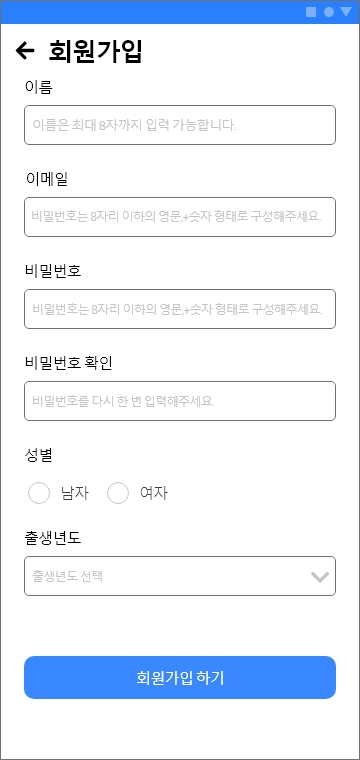
\includegraphics[scale=0.32]{assets/회원가입1.jpg}} \\
    \item[] It consists of fields that receive the name, email, password, and password check. \\
    \begin{itemize}
    \item[-] The name must be entered in 8 characters or less, and we notify you in advance that the name is a necessary element to be called within the app. \\ \\
    \item[-] The e-mail will be exposed to the phrase asking you to follow the e-mail format and enter it.
    \\ \\
    \item[-] The password will be exposed in a combination of English and numbers of less than 8 digits.
    \\ \\
    \item[-] In the case of password verification, the same phrase as the password entered above will be exposed.
    \\
    \item[-] If an input value that does not match the rules is entered in the field, the field is processed red, and a warning statement is exposed at the bottom.

\break
    
          \begin{enumerate} 
          \item Phrases when invalid \\ \\
            \centerline{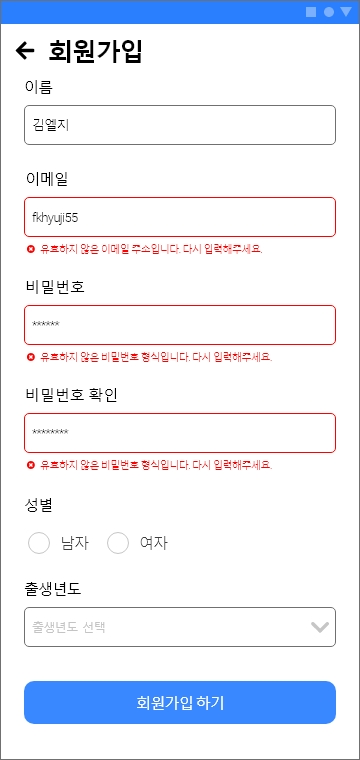
\includegraphics[scale=0.28]{assets/회원가입3.jpg}}
          \begin{enumerate}
          \item The name is not valid. Please input it again.
          \item This is an invalid email format. Please input it again.
          \item This is an invalid password format. Please input it again.
          \item The password does not match. Please input it again.
        \end{enumerate}
    \item[-] \\ If an input value that matches the rule is entered, the field is processed in green, and the phrase "valid value" is exposed at the bottom. \\
    \item Phrases when valid \\ \\ \\
    \centerline{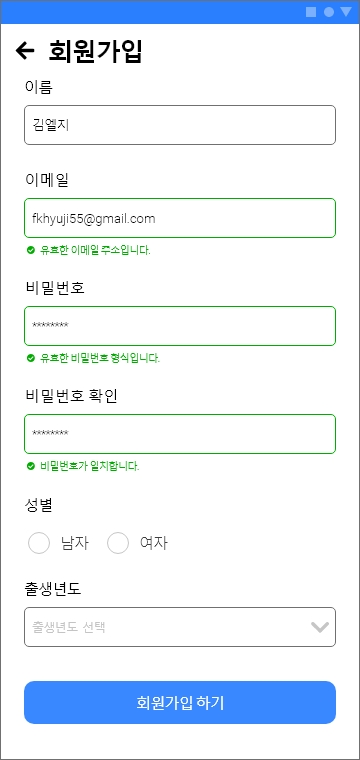
\includegraphics[scale=0.28]{assets/회원가입2.jpg}}
    \begin{enumerate}
\item This is a valid name.
\item This is a valid email format.
\item This is a valid password format.
\item The password matches.
    \end{enumerate}
        \end{enumerate}
          \end{itemize}
    \item Pop-up \\\\
    \centerline{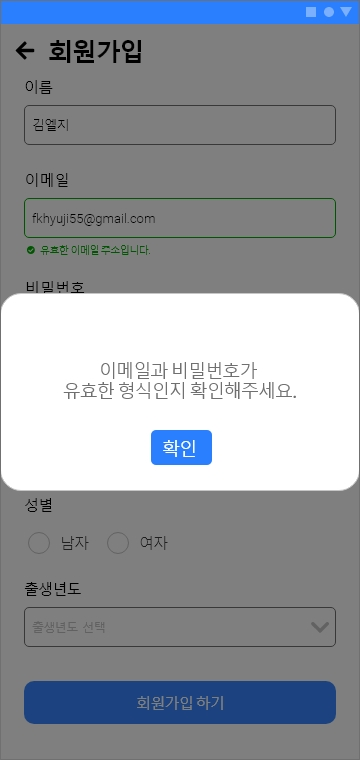
\includegraphics[scale=0.32]{assets/회원가입4.jpg}}
    \begin{itemize}
        \item[] \\ \\ If you click the Sign-up button before the form is not completed, a pop-up with ’All values have not been entered. Please complete the input.' comment is displayed at the bottom. When you click the gray area or 'x button' or 'OK button', the pop-up will end and the previous one will be exposed again.\\ 
    \end{itemize}
    \item Completed page \\ \\
    \centerline{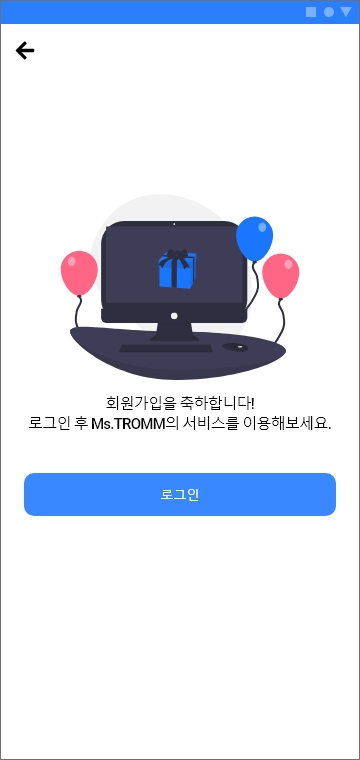
\includegraphics[scale=0.32]{assets/회원가입5.jpg}}
        \begin{itemize}
        \item[] This page is exposed when membership is completed. Click the login button to go to the login screen.
    \end{itemize}
    \end{enumerate}

\subsection{Main Page}
\begin{itemize}
    \item[] When the login is completed, the main page is exposed. When a user with no login record logs in for the first time, the questionnaire page is exposed instead of the main page.
    \item[] At home, you can check four items: notification, today's weather, today's recommendation, basic styler control, and our house status. Also, there is a connection button with a styler or smart mirror, so it is possible to easily check and connect the connection status.\\  
\end{itemize}
\begin{enumerate}
    \item Survey(first time to entry) 
    \begin{enumerate}
    \item Information page \\ \\ \\
    \centerline{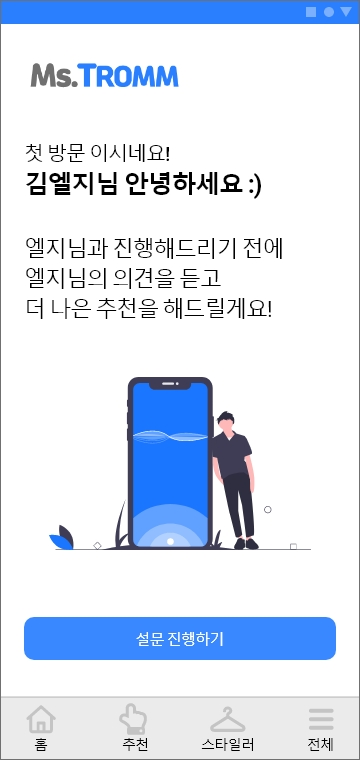
\includegraphics[scale=0.32]{assets/설문지1.jpg}}
    \begin{itemize}
        \item[] \\ \\ This is a page that guides the survey. The survey progress button is exposed at the bottom. The survey consists of contents that will be conducted because it is helpful for the recommendation. \\ \\ \\ \\ \\ \\ \\ \\ \\ \\ \\ \\ \\ \\ \\ 

    \end{itemize} 
        \item Survey page \\ \\ \\
        \leftline{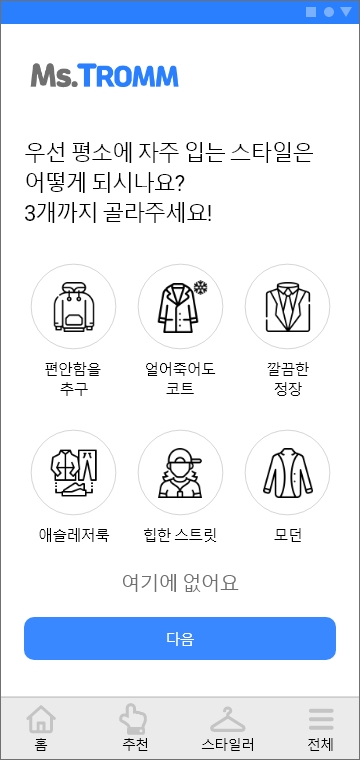
\includegraphics[scale=0.15]{assets/설문지2.jpg}
                   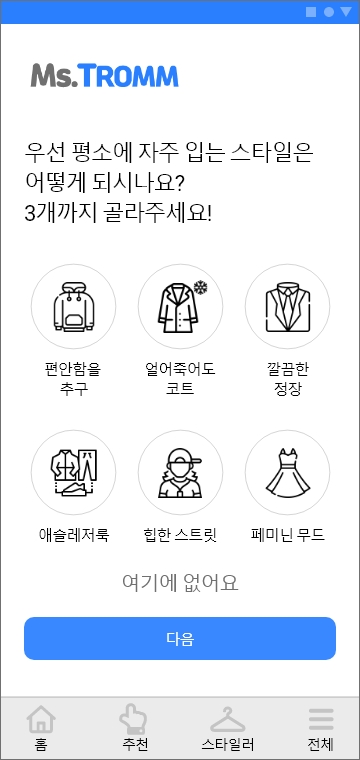
\includegraphics[scale=0.15]{assets/설문지3.jpg}
                   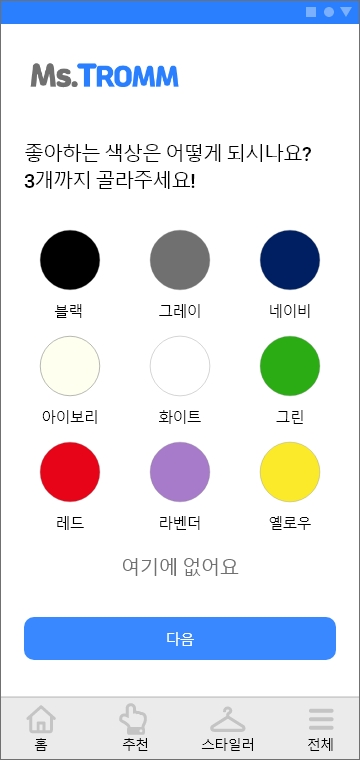
\includegraphics[scale=0.15]{assets/설문지4.jpg}
                    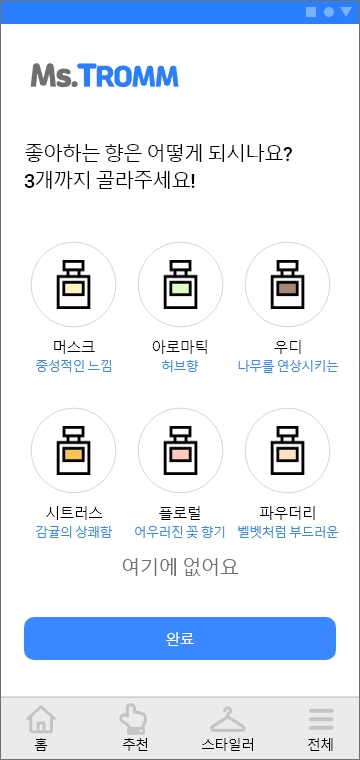
\includegraphics[scale=0.15]{assets/설문지5.jpg}}
    \begin{itemize}
        \item[] \\ \\ This is a survey to increase the recommended accuracy of Ms. TROMM. The survey consists of questions about three elements (a style you usually wear often, a favorite color, and a favorite scent). In the case of frequently worn styles, different questions are provided depending on the gender entered when signing up as a member.\\
        \break
        \end{itemize} 
        \item Pop-up\\ \\
            \centerline{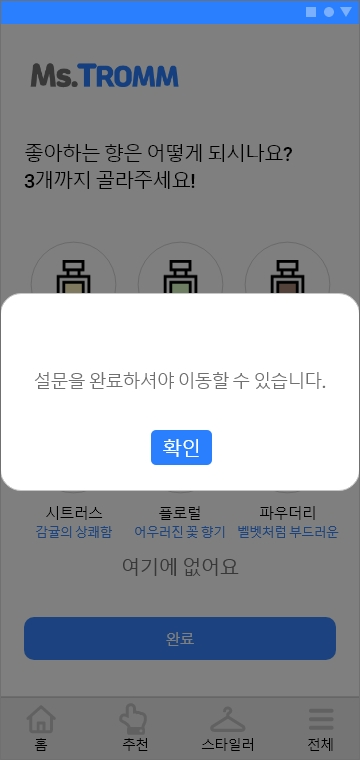
\includegraphics[scale=0.32]{assets/설문지6.jpg}}
    \begin{itemize}
        \item[]  This is a pop-up that is exposed at the bottom of the questionnaire when you try to leave the page. "You must complete the survey to move!" will be displayed. When you click the gray area, 'x button', or 'OK button', the pop-up will end and the survey page will be exposed again.\\ \\ \\
        \end{itemize} 

    \item Completed page \\ \\ \\
    \centerline{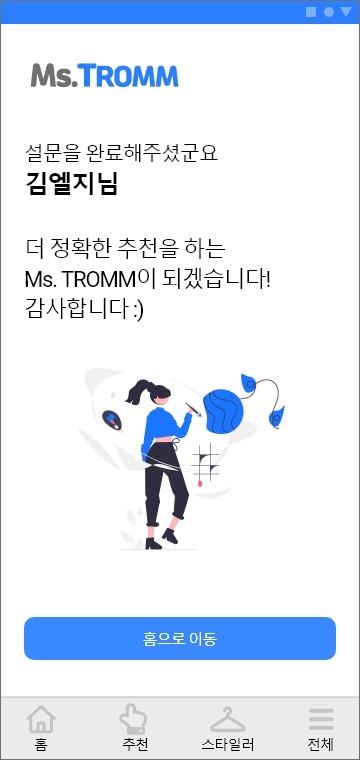
\includegraphics[scale=0.32]{assets/설문지7.jpg}}
    \begin{itemize}
        \item[] This page appears when you complete the survey. The "Move to Home" button is exposed at the bottom. When clicking the button, go to Home.\\ \\ \\ \\
        \end{itemize} 
\end{enumerate}
\item Home(Main page)\\ \\
\centerline{\includegraphics[scale=0.32]{assets/홈4.jpg}}
\begin{itemize}
    \item[] Home shows basic functions in the app at once.\\\\
\end{itemize}
 \begin{enumerate}
 \centerline{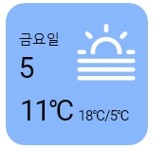
\includegraphics[scale=1]{assets/일반 위젯.jpg}}
 \item[-]Indicate today's date and current weather. \\\\
 \leftline{
\includegraphics[scale=1]{assets/오늘의 추천 위젯.jpg}}
 \item[-] Today's recommendation item is provided in the form of a preview of the recommendation that the user has set as the default recommendation.\\\\
 \item[-] Styler control items allow you to check the connection and connection status with the Styler/Smart Mirror and support the pause/react button when the Styler is operated. It also displays the remaining time until the styler operation stage and shutdown.\\\\
 \leftline{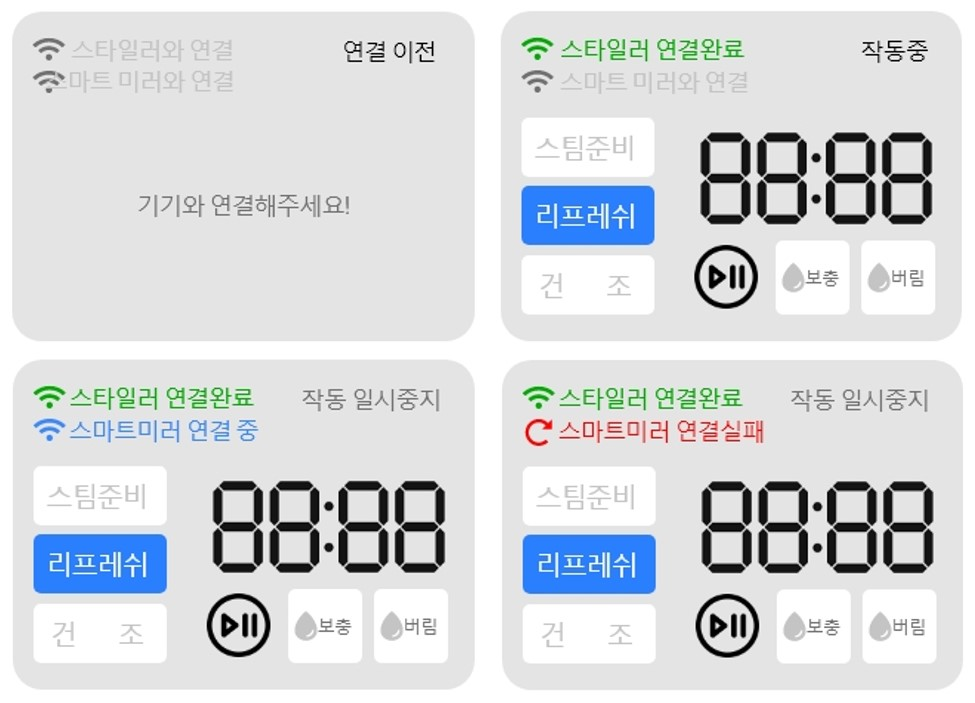
\includegraphics[scale=0.40]{assets/스타일러 제어 위젯.jpg}}
 \break
 \item[-] \\ \\ If the styler/smart mirror is not connected, when clicked, it will be changed to a message indicating that the connection is underway and the color will be changed.\\ \\ \\ \\ \\
 \item[-] If the connection to the styler/smart mirror fails, it will be changed to a comment indicating the connection failure and the color will be changed. \\ \\
 \leftline{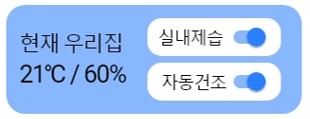
\includegraphics[scale=0.75]{assets/현재 우리집 위젯.jpg}}
 \item[-] \\ \\ Current status of our home menu displays the temperature and humidity of the house, and buttons are located to turn on indoor dehumidification and automatic drying functions.\\ \\
 \end{enumerate}
 \item Bottom Nav \\ \\ \\ \\
 \centerline{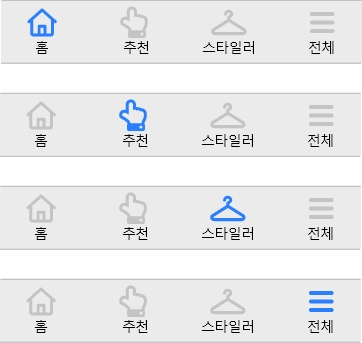
\includegraphics[scale=0.5]{assets/하단 nav.jpg}}
 \break
 \begin{itemize}
    \item[] This is the bottom nav in the app. It consists of home, recommendation, styler, and whole, and when clicked, the picture is activated and goes to the page.
\end{itemize}
\end{enumerate}

\subsection{Pop-up} \\ \\
\begin{itemize}
    \item[] Notifications occurring in the app occur as pop-ups and can be found in the notification menu. You can enter the notification menu at the top of the home screen.\\ \\ \\ \\ \\
\end{itemize}

\break

\begin{enumerate}
    \item Today's recommendation notification \\
    \centerline{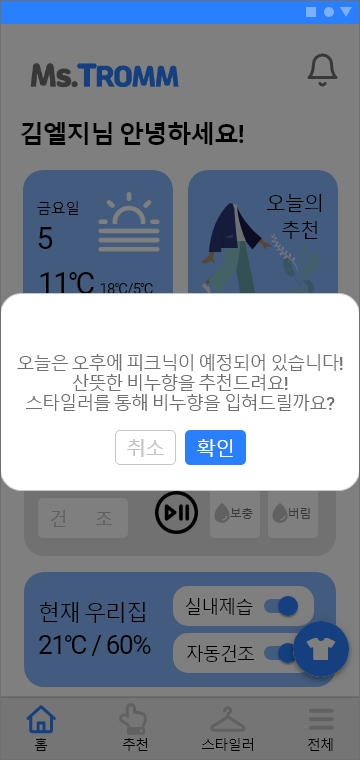
\includegraphics[scale=0.18]{assets/오늘의 추천 팝업1.jpg}
    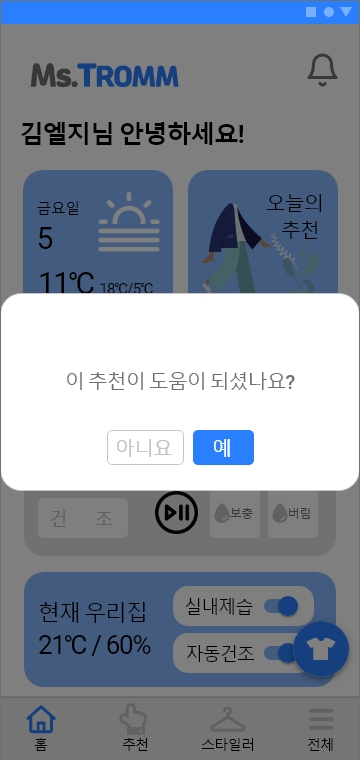
\includegraphics[scale=0.18]{assets/오늘의 추천 팝업2.jpg}
    \includegraphics[scale=0.18]{assets/오늘의 추천 팝업3.jpg}}
    \begin{itemize}
    \item[] Today's recommendation is caused by a pop-up notification. After checking the notification, a notification occurs to select whether the recommendation was helpful, and the recommendation termination popup is exposed when responding. Data from the notification asking for recommendation help is recorded on the server, and more personalized recommendations are made using it.\\ 
\end{itemize}
\item Control recommendation notification \\
\centerline{\includegraphics[scale=0.18]{assets/제어추천 팝업1.jpg}
            \includegraphics[scale=0.18]{assets/제어추천 팝업2.jpg}}
\break
    \begin{itemize}
    \item[] This is a notification that occurs when there is a lack of water in the styler or when water needs to be discarded. \\
\end{itemize}
\centerline{\includegraphics[scale=0.18]{assets/제어추천 팝업3.jpg}
            \includegraphics[scale=0.18]{assets/제어추천 팝업4.jpg}}
\break
    \begin{itemize}
    \item[] This is a notification of indoor dehumidification and automatic drying control that occur when indoor humidity exceeds 40. \\ \\
\end{itemize}
     \item Weather notification\\ \\
     \centerline{\includegraphics[scale=0.30]{assets/날씨 추천 팝업.jpg}}
    \begin{itemize}
    \item[] \\ \\ \\ \\A pop-up notification occurs based on the weather. For example, if there's a rain forecast, you'll be notified to bring an umbrella..\\
\end{itemize}
     \item Schedule notification \\ \\
     \centerline{\includegraphics[scale=0.30]{assets/일정 추천 팝업.jpg}}
    \begin{itemize}
    \item[] \\ \\ \\ \\ A pop-up notification occurs based on the schedule. For example, if you have an interview, you will be notified of the interview cheering comment\\
\end{itemize}
\end{enumerate}

\subsection{Notification} \\ \\
\begin{itemize}
    \item[] This is a menu in which the pop-up notification list that has occurred is recorded.\\ \\ \\
\end{itemize}
\begin{enumerate}
 \centerline{\includegraphics[scale=0.32]{assets/알림1.jpg}}
 \item[-]\\This is the initial notification screen. Comments related to push alarm setting appear. \\\\\\\\
 \centerline{\includegraphics[scale=0.32]{assets/알림2.jpg}}
 \item[-] This is a screen that is exposed when there is no notification history after replacing the push alarm setting to ON.\\\\\\\\
 \centerline{\includegraphics[scale=0.32]{assets/알림3.jpg}}
 \item[-] \\\\ This is a screen that is exposed when there is a notification list.\\\\\\\\\\\\
\centerline{\includegraphics[scale=0.25]{assets/알림4.jpg}
            \includegraphics[scale=0.25]{assets/알림5.jpg}}
 \item[-] \\When you click on the notification list, the body containing the notification is exposed.\\\\\\\\\\\
 \end{enumerate}

\subsection{Recommendation}
\begin{itemize}
\item[] It's a menu that shows the recommendations. There are a total of two recommended criteria, including today's schedule and control. You can select the recommendation criteria at the top, and if you click the recommendation part of the recommendation, a pop-up related to fragrance use will occur.\\
\end{itemize}
    \begin{enumerate}
    \item Button description(first time to entry) \\ \\
    \centerline{\includegraphics[scale=0.32]{assets/추천1.jpg}}
        \begin{itemize}
    \item[] When entering the recommendation menu for the first time, a page informing you of the basic functions of the buttons in the recommendation menu is exposed. It ends when you click on the gray area. \\
\end{itemize}
     \item Today's Recommendation \\ \\
     \centerline{\includegraphics[scale=0.32]{assets/추천2.jpg}}
    \begin{itemize}
    \item[] \\ \\ \\ \\ This menu exposes today's recommendations using calendars and weather APIs. Comments and recommendations suitable for the date will be exposed.\\
\end{itemize}
       \item Control Recommendation \\ \\ \\
       \centerline{\includegraphics[scale=0.32]{assets/추천3.jpg}}
       \break
           \begin{itemize}
    \item[] It is a menu that provides recommendations related to the clothing and home environment in the styler.\\\\\\
\end{itemize}
     \item Pop-up related to fragrance use \\ \\
     \centerline{\includegraphics[scale=0.25]{assets/추천4.jpg}
                \includegraphics[scale=0.25]{assets/추천5.jpg}}
    \begin{itemize}
    \item[] \\ \\ \\ \\ This is a pop-up that is exposed when you click the fragrance recommendation part. Ask questions about applying the Styler Introductory Application, and forward the sheet activation command to the Styler when the user wants to apply the fragrance.\\
\end{itemize}
\end{enumerate}

\subsection{Styler}  \\ 
\centerline{\includegraphics[scale=0.32]{assets/스타일러4.jpg}}
This is a menu where you can control the styler. Control buttons on the styler are exposed.
 \begin{enumerate}
\centerline{\includegraphics[scale=0.32]{assets/스타일러1.jpg}}
 \item[-]This is a page that appears when not connected to the styler. \\\\
\centerline{\includegraphics[scale=0.5]{assets/제어 버튼1.jpg}} \\ \\
\centerline{\includegraphics[scale=0.5]{assets/제어 버튼2.jpg}} \\ \\
\centerline{\includegraphics[scale=0.5]{assets/제어 버튼3.jpg}} \\ \\
 \item[-]It's related to the operation of the styler. There are Styler power-on, power-off, start operation, stop operation buttons, and reservation buttons. If the styler is running, it displays which function is running. \\\\
  \centerline{\includegraphics[scale=0.5]{assets/스타일러 버튼.jpg}}
 \item[-]It's a menu that can be operated by the styler. It supports a total of six functional operations \\\\
\centerline{\includegraphics[scale=0.3]{assets/스타일링 선택.jpg}
            \includegraphics[scale=0.3]{assets/섬세건조 선택.jpg}} \\ \\
\centerline{\includegraphics[scale=0.3]{assets/고급의류 선택.jpg}
            \includegraphics[scale=0.3]{assets/스팀살균 선택.jpg}} \\ \\
 \item[-]Details of the course will be exposed when each button is clicked. \\\\
   \centerline{\includegraphics[scale=0.32]{assets/스타일러7.jpg}}
 \item[-]This is a pop-up that is exposed when another styler menu is pressed while the styler is running. \\\\
 \end{enumerate}
 
\subsection{My Closet}  \\
The button to enter my closet menu continues to be exposed to a floating action button within the app.
\begin{enumerate}
\item My Closet\\ \\
 \begin{enumerate}
 \centerline{\includegraphics[scale=0.32]{assets/내 옷장1.jpg}}
 \item[-]The registration date of the clothes and the date you put them in the styler most recently are displayed. The clothes bookmarked at the top are currently in the styler. \\\\
 \item[-]Clothes that need to be turned around in the styler will be guided above. We need a styler in order of importance. - How about a styler?This outfit is okay. \\\\
 \centerline{\includegraphics[scale=0.32]{assets/내 옷장2.jpg}}
 \item[-] When you click on the bottom of the list, detailed information about the clothes appears. The information that appears is the registration date, the last styler working day, and the contents that were registered when registering clothes.\\\\
 \end{enumerate}
 
 \item Register New clothes\\ \\
 \begin{enumerate}
    \centerline{\includegraphics[scale=0.24]{assets/새 옷 등록하기1.jpg}
    \includegraphics[scale=0.24]{assets/새 옷 등록하기2.jpg}}
 \item[-]It's a menu to register new clothes. At first, the part where you put the picture of the clothes and the name input field are exposed. \\\\
 \centerline{\includegraphics[scale=0.32]{assets/새 옷 등록하기3.png}}
 \item[-]Next, fields where you can enter colors, styling courses, high-end drying courses, and sterilization are exposed. \\\\
  \centerline{\includegraphics[scale=0.32]{assets/새 옷 등록하기4.png}}
 \item[-]This is a screen where a guide phrase for designating no category is exposed as a pop-up. \\\\
  \centerline{\includegraphics[scale=0.32]{assets/새 옷 등록하기5.png}}
 \item[-]This is a pop-up announcing the completion of the procedure for registering new clothes. \\\\
 \end{enumerate}
 
 \item Register New clothes\\ \\
 \begin{enumerate}
    \centerline{\includegraphics[scale=0.24]{assets/새 옷 등록하기1.jpg}
    \includegraphics[scale=0.24]{assets/새 옷 등록하기2.jpg}}
    \item[-]It's a menu to register new clothes. At first, the part where you put the picture of the clothes and the name input field are exposed. \\\\
    \centerline{\includegraphics[scale=0.32]{assets/새 옷 등록하기3.png}}
    \item[-]Next, fields where you can enter colors, styling courses, high-end drying courses, and sterilization are exposed. \\\\
    \centerline{\includegraphics[scale=0.32]{assets/새 옷 등록하기4.png}}
    \item[-]This is a screen where a guide phrase for designating no category is exposed as a pop-up. \\\\
    \centerline{\includegraphics[scale=0.32]{assets/새 옷 등록하기5.png}}
    \item[-]This is a pop-up announcing the completion of the procedure for registering new clothes. \\\\
    \end{enumerate}
\end{enumerate}

\subsection {All} \\
This is a menu where you can check the general information of the app. You can check the subscription information and version information terms and conditions, and there is a menu that allows you to change the default settings in the app.
\begin{enumerate}
    \item Login form screen \\ \\
    \centerline{\includegraphics[scale=0.32]{assets/전체.jpg}}
    \begin{itemize}
    \item[] Version information is displayed in this menu page. \\
    \end{itemize}
    \item My information \\\\
    \centerline{\includegraphics[scale=0.32]{assets/내 정보1.jpg}}
    \begin{itemize}
    \item[] This is a menu where you can check the information you entered when signing up. If you want to change the information, click the Change button at the bottom to see the Change screen. \\ \\
    \end{itemize}
    \centerline{\includegraphics[scale=0.32]{assets/내 정보2.jpg}}
    \begin{itemize}
    \item[] After pressing Change, the screen is displayed. You can modify the information you entered when signing up. \\ \\
    \end{itemize}
    
    \break
    
    \item Terms and Conditions \\ \\ \\
    \centerline{\includegraphics[scale=0.32]{assets/개인정보약관.jpg}}
    \begin{itemize}
    \item[]You can check the terms and conditions of using personal information. \\ \\ 
    \end{itemize}
\end{enumerate}

\section{ARCHITECTURE DESIGN AND IMPLEMENTATION}

\subsection{Overall Architecture}
\centerline{\includegraphics[scale=0.15]{assets/Overall architecture.jpg}}
\\ \\ \\ We have three parts consisting of our application ‘Ms. TROMM’. First part is ‘Flutter’ which is for our frontend. It mainly reacts with the client(user) part. This will help us our overall application containing several functions and designs. For our backend which mainly reacts with the server, we use Flask and SQL Alchemy. Flask adopted it because it can build and develop back-and-server light and fast. In addition, through SQL Alchemy, the database can be object-oriented and SQL can be handled with Python. Last part is MySQL and Heroku which is for server. MySQL is used to remotely manage databases, and MySQL is connected to Heroku Service Part, a server that provides free hosting up to certain traffic.\\ \\

\subsection{Directory organization}
This is the table which shows directory, file name and module name.\\

\begin{table} [h]
    \centering
    \begin{tabular}{l|l|l}
    \hline
    \textit{\textbf{Directory}} & \textit{\textbf{File Name}} & \textit{\textbf{Module}}
     & & & \\ \hline
    \begin{tabular}[c]{@{}l@{}}\\Ms-TROMM/\\Ms.TROMM\_Frontend/\\\\\\\\\\\\\\\\\\\\\\\\\\\\\\\end{tabular} & \begin{tabular}[c]{@{}l@{}}\\.firebaserc\\\\.gitignore\\\\.metadata\\\\README.md\\\\analysis_options.yaml\\\\.firebase.json\\\\pubspec.lock\\\\pubspec.yaml\\\\\end{tabular} 
    & \begin{tabular}[c]{@{}l@{}}\\Frontend (Flutter) \\\\\\\\\\\\\\\\\\\\\\\\\\\\\\\\\end{tabular} \\ \hline
    \begin{tabular}[c]{@{}l@{}}\\Ms-TROMM/\\Ms.TROMM\_Frontend/\\.firebase/\\\\\end{tabular} & \begin{tabular}[c]{@{}l@{}}\\hosting.YnVpbGRcd2Vi\\.cache\\\\\\\end{tabular} 
    & \begin{tabular}[c]{@{}l@{}}\\Frontend (Flutter)\\\\\\\\\end{tabular} \\ \hline
    \begin{tabular}[c]{@{}l@{}}\\Ms-TROMM/\\Ms.TROMM\_Frontend/\\android/app/src/\\main/res/drawable\\\\\end{tabular} & \begin{tabular}[c]{@{}l@{}}\\background.png\\\\launch_background.xml\\\\\\\end{tabular} 
    & \begin{tabular}[c]{@{}l@{}}\\Frontend (Flutter)\\\\\\\\\\\end{tabular} \\ \hline
    \begin{tabular}[c]{@{}l@{}}\\Ms-TROMM/\\Ms.TROMM\_Frontend/\\android/app/src/\\main/res/values\\\\\end{tabular} & \begin{tabular}[c]{@{}l@{}}\\styles.xml\\\\\\\\\\\end{tabular} 
    & \begin{tabular}[c]{@{}l@{}}\\Frontend (Flutter)\\\\\\\\\\\end{tabular} \\ \hline
    \begin{tabular}[c]{@{}l@{}}\\Ms-TROMM/\\Ms.TROMM\_Frontend/\\db/\\\\\end{tabular} & \begin{tabular}[c]{@{}l@{}}\\schema.sql\\\\\\\\\end{tabular} & \begin{tabular}[c]{@{}l@{}}\\Frontend (Flutter)\\\\\\\\\end{tabular} \\ \hline
    \begin{tabular}[c]{@{}l@{}}\\Ms-TROMM/\\Ms.TROMM\_Frontend/\\android/app/src/\\main/res/values\\\\\end{tabular} & \begin{tabular}[c]{@{}l@{}}\\styles.xml\\\\\\\\\\\end{tabular} 
    & \begin{tabular}[c]{@{}l@{}}\\Frontend (Flutter)\\\\\\\\\\\end{tabular} \\ \hline
    \begin{tabular}[c]{@{}l@{}}\\Ms-TROMM/\\Ms.TROMM\_Frontend/\\ios/Runner\\\\\\\end{tabular} & \begin{tabular}[c]{@{}l@{}}\\AppDelegate.swift\\\\info.plist\\\\Runner-Bridging-Header.h\\\\\end{tabular} & \begin{tabular}[c]{@{}l@{}}\\Frontend (Flutter)\\\\\\\\\\\\\end{tabular} \\ \hline
    \end{tabular}
\end{table}

\begin{table} [p]
    \centering
    \begin{tabular}{l|l|l}
    \hline 
    \begin{tabular}[c]{@{}l@{}}\\Ms-TROMM/\\Ms.TROMM\_Frontend/\\ios/Runner\\Assets.xcassets/\\LaunchBackground\\.imageset/\\\\\end{tabular} & \begin{tabular}[c]{@{}l@{}}\\Contents.json\\\\background.png\\\\\\\\\\\end{tabular} & \begin{tabular}[c]{@{}l@{}}\\Frontend (Flutter)\\\\\\\\\\\\\\\end{tabular} \\ \hline
    \begin{tabular}[c]{@{}l@{}}\\Ms-TROMM/\\Ms.TROMM\_Frontend/\\ios/Runner\\Assets.xcassets/\\LaunchImage\\.imageset/\\\\\end{tabular} & \begin{tabular}[c]{@{}l@{}}\\Contents.json\\\\LaunchImage.png\\\\\\\\\\\end{tabular} & \begin{tabular}[c]{@{}l@{}}\\Frontend (Flutter)\\\\\\\\\\\\\\\end{tabular} \\ \hline
    \begin{tabular}[c]{@{}l@{}}\\Ms-TROMM/\\Ms.TROMM\_Frontend/\\ios/Runner\\Base.lproj/\\\\\end{tabular} & \begin{tabular}[c]{@{}l@{}}\\LaunchScreen.storyboard\\\\Main.storyboard\\\\\\\end{tabular} & \begin{tabular}[c]{@{}l@{}}\\Frontend (Flutter)\\\\\\\\\\\end{tabular} \\ \hline
    \begin{tabular}[c]{@{}l@{}}\\Ms-TROMM/\\Ms.TROMM\_Frontend/\\lib/\\\\\end{tabular} & \begin{tabular}[c]{@{}l@{}}\\main.dart\\\\\\\\\end{tabular} & \begin{tabular}[c]{@{}l@{}}\\Frontend (Flutter)\\\\\\\\\end{tabular} \\ \hline
    \begin{tabular}[c]{@{}l@{}}\\Ms-TROMM/\\Ms.TROMM\_Frontend/\\lib/local\_db/\\\\\end{tabular} & \begin{tabular}[c]{@{}l@{}}\\database\_example.dart\\\\shared\_pref.dart\\\\\end{tabular} & \begin{tabular}[c]{@{}l@{}}\\Frontend (Flutter)\\\\\end{tabular} \\ \hline
    \begin{tabular}[c]{@{}l@{}}\\Ms-TROMM/\\Ms.TROMM\_Frontend/\\lib/models/\\\\\\\\\\\\\\\end{tabular} & \begin{tabular}[c]{@{}l@{}}\\album.dart\\\\connectable.dart\\\\smart\_mirror.dart\\\\styler.dart\\\\user.dart\\\\\end{tabular} & \begin{tabular}[c]{@{}l@{}}\\Frontend (Flutter)\\\\\\\\\\\\\\\\\\\end{tabular} \\ \hline
    \begin{tabular}[c]{@{}l@{}}\\Ms-TROMM/\\Ms.TROMM\_Frontend/\\lib/ui/authentication/\\\\\\\\\\\\\\\\\\\\\\\\\end{tabular} & \begin{tabular}[c]{@{}l@{}}\\change\_password.dart\\\\login.dart\\\\signup.dart\\\\signup\_done.dart\\\\tutorial.dart\\\\utils.dart\\\\validators.dart\\\\\end{tabular} & \begin{tabular}[c]{@{}l@{}}\\Frontend (Flutter)\\\\\\\\\\\\\\\\\\\\\\\\\\\\\end{tabular} \\ \hline
    \begin{tabular}[c]{@{}l@{}}\\Ms-TROMM/\\Ms.TROMM\_Frontend/\\lib/ui/home/\\\\\end{tabular} & \begin{tabular}[c]{@{}l@{}}\\alert\_page.dart\\\\home.dart\\\\\end{tabular} & \begin{tabular}[c]{@{}l@{}}\\Frontend (Flutter)\\\\\\\\\end{tabular} \\ \hline
    \end{tabular}
\end{table}

\begin{table} [t]
    \centering
    \begin{tabular}{l|l|l} \hline
    \begin{tabular}[c]{@{}l@{}}\\\end{tabular} & \begin{tabular}[c]{@{}l@{}}\\moisture\_box.dart\\\\recommendation\_box\\.dart\\\\styler\_control\_box\\.dart\\\\weather_box.dart\\\\\end{tabular} & \begin{tabular}[c]{@{}l@{}}\\Frontend (Flutter)\\\\\\\\\\\\\\\\\\\\\end{tabular} \\ \hline
    \begin{tabular}[c]{@{}l@{}}\\Ms-TROMM/\\Ms.TROMM\_Frontend/\\lib/ui/settings/\\\\\end{tabular} & \begin{tabular}[c]{@{}l@{}}\\settings.dart\\\\\\\\\end{tabular} & \begin{tabular}[c]{@{}l@{}}\\Frontend (Flutter)\\\\\\\\\end{tabular} \\ \hline
    \begin{tabular}[c]{@{}l@{}}\\Ms-TROMM/\\Ms.TROMM\_Frontend/\\lib/ui/styler/\\\\\end{tabular} & \begin{tabular}[c]{@{}l@{}}\\styler.dart\\\\styler2.dart\\\\\end{tabular} & \begin{tabular}[c]{@{}l@{}}\\Frontend (Flutter)\\\\\\\\\end{tabular} \\ \hline
    \begin{tabular}[c]{@{}l@{}}\\Ms-TROMM/\\Ms.TROMM\_Frontend/\\lib/ui/survey/\\\\\\\\\\\\\\\\\end{tabular} & \begin{tabular}[c]{@{}l@{}}\\survey\_done.dart\\\\survey\_main.dart\\\\survey\_step\_1.dart\\\\survey\_step\_2.dart\\\\survey\_step\_3.dart\\\\\end{tabular} & \begin{tabular}[c]{@{}l@{}}\\Frontend (Flutter)\\\\\\\\\\\\\\\\\\\\\end{tabular} \\ \hline
    \begin{tabular}[c]{@{}l@{}}\\Ms-TROMM/\\Ms.TROMM\_Frontend/\\lib/ui/widgets/\\\\\\\\\\\\\\\end{tabular} & \begin{tabular}[c]{@{}l@{}}\\alert\_dialog.dart\\\\logo.dart\\\\spacer.dart\\\\tromm\_button.dart\\\\\end{tabular} & \begin{tabular}[c]{@{}l@{}}\\Frontend (Flutter)\\\\\\\\\\\\\\\\\\\end{tabular} \\ \hline
    \begin{tabular}[c]{@{}l@{}}\\Ms-TROMM/\\Ms.TROMM\_Frontend/\\web/\\\\\end{tabular} & \begin{tabular}[c]{@{}l@{}}\\index.html\\\\\\\\\end{tabular} & \begin{tabular}[c]{@{}l@{}}\\Frontend (Flutter)\\\\\\\\\end{tabular} \\ \hline
    \begin{tabular}[c]{@{}l@{}}\\Ms-TROMM/\\Ms.TROMM\_Frontend/\\web/splash\\\\\end{tabular} & \begin{tabular}[c]{@{}l@{}}\\style.css\\\\\\\\\end{tabular} & \begin{tabular}[c]{@{}l@{}}\\Frontend (Flutter)\\\\\\\\\end{tabular} \\ \hline
    \begin{tabular}[c]{@{}l@{}}\\Ms-TROMM/\\Ms.TROMM\_Backend/\\\\\\\\\\\\\\\end{tabular} & \begin{tabular}[c]{@{}l@{}}\\.gitignore\\\\requirements.txt\\\\README.md\\\\wsgi.py\\\\\end{tabular} 
    & \begin{tabular}[c]{@{}l@{}}\\Backend\\(Flask+SQL Alchemy)\\\\\\\\\\\\\\\end{tabular} \\ \hline
    \end{tabular}
\end{table}

\begin{table} [t]
    \centering
    \begin{tabular}{l|l|l}
    \hline
    \begin{tabular}[c]{@{}l@{}}\\Ms-TROMM/\\Ms.TROMM\_Backend/\\flaskr/\\\\\\\end{tabular} & \begin{tabular}[c]{@{}l@{}}\\Swg.py\\\\clothe.csv\\\\dataset.csv\\\\\end{tabular} 
    & \begin{tabular}[c]{@{}l@{}}\\Backend\\(Flask+SQL Alchemy)\\\\\\\end{tabular} \\ \hline
    \begin{tabular}[c]{@{}l@{}}\\Ms-TROMM/\\Ms.TROMM\_Backend/\\flaskr/\\\\\\\end{tabular} & \begin{tabular}[c]{@{}l@{}}\\Swg.py\\\\clothe.csv\\\\dataset.csv\\\\main.py\\\\swagger.yml\\\\\end{tabular} 
    & \begin{tabular}[c]{@{}l@{}}\\Backend\\(Flask+SQL Alchemy)\\\\\\\end{tabular} \\ \hline 
    \begin{tabular}[c]{@{}l@{}}\\Ms-TROMM/\\Ms.TROMM\_Backend/\\flaskr/models/\\\\\\\\\\\\\\\\\\\\\\\\\\\\\\\\\\\\\\\\\\\end{tabular} & \begin{tabular}[c]{@{}l@{}}\\\_init\_.py\\\\clothes.py\\\\clothes\_combination.py\\\\control.py\\\\mirror.py\\\\recommendation.py\\\\scent.py\\\\schedule.py\\\\styler.py\\\\styler\_alert.py\\\\user.py\\\\user\_preference.py\\\\\end{tabular} 
    & \begin{tabular}[c]{@{}l@{}}\\Backend\\(Flask+SQL Alchemy) \\\\\\\\\\\\\\\\\\\\\\\\\\\\\\\\\\\\\\\\\\\\\end{tabular} \\ \hline
    \begin{tabular}[c]{@{}l@{}}\\Ms-TROMM/\\Ms.TROMM\_Backend/\\\\\end{tabular} & \begin{tabular}[c]{@{}l@{}}\\Procfile\\\\install.md\\\\\end{tabular} 
    & \begin{tabular}[c]{@{}l@{}}\\DB\\(MySQL+Heroku)\\\\\end{tabular} \\ \hline
    \begin{tabular}[c]{@{}l@{}}\\Ms-TROMM/\\Ms.TROMM\_Backend/\\flaskr\\\\\end{tabular} & \begin{tabular}[c]{@{}l@{}}\\settings.py\\\\\\\\\end{tabular} 
    & \begin{tabular}[c]{@{}l@{}}\\DB\\(MySQL+Heroku)\\\\\\\end{tabular} \\ \hline
    
    \begin{tabular}[c]{@{}l@{}}\\Ms-TROMM/\\Ms.TROMM\_document/\\\\\\\end{tabular} & \begin{tabular}[c]{@{}l@{}}\\Ms.TROMM.pdf\\\\Ms.TROMM.tex\\\\\end{tabular} 
    & \begin{tabular}[c]{@{}l@{}}\\Documentation\\\\\\\\\end{tabular} \\ \hline
    \end{tabular}
    \renewcommand{\thetable}{\arabic{table}}
    \caption{Directory of Ms. TROMM}
    \label{table}
\end{table}

\textcolor[rgb]{1,1,1}{(This is blank)}\\\\\\\\\\\\\\\\\\\\\\\\\\\\\\\\\\\\\

\subsection{Part 1: Flutter (Frontend)}
\begin{enumerate}
    \item Purpose\\
    To develop Ms.TROMM, a cross-platform that can be developed in both Android and iOS environments, we used Flutter, a web/app cross-platform framework developed by Google based on the Dart language. In the case of Ms.TROMM developed with Flutter, it can be used in both web and app environments. The advantage of developing Ms.TROMM is that it can be developed in a familiar environment among the existing iOS or Android development environments, such as Android Studio or Xcode. In the case of Ms.TROMM, it is an artificial intelligence software that provides better recommendations while accumulating data through learning, so it is important to provide an environment that can be used by more users. Therefore, Flutter was adopted as a front-end development environment to provide a better experience for both developers and users. \\ \\
    \item Functionality\\
    Ms.TROMM's front-end made with Flutter requests JSON-type data processed by the back-end itself (or processed from the database) from the back-end and serves to show Ms.TROMM users to use it easily. In addition, the information received from the user is delivered to the back-end server and stored (updated) in the database, or data is provided for the back-end server to process. In other words, users can communicate with the backend server of Ms.TROMM through the frontend of Ms.TROMM as well as with the systems of LG Styler and LG Smart Mirror. Users can get a better experience for Ms.TROMM and LG Electronics from the user-friendly front-end of Ms.TROMM. \\ \\
    \item Location of source code: \\: Ms-TROMM/MsTROMM\_Frontend/ \\ \\
    \item Class component: - \\
    \item Where it is taken from\\
    Install the Flutter SDK first. Environmental variables must be set to use the plotter command. If you type environmental variables in the window search box, you will see "Edit System Environment Pile" and click it. Find and correct the variable 'PATH' in the user variable and put the Flutter SDK in the BIN path. Run the flutter console and enter the flutter doctor command to verify that the conditions for executing the flutter are satisfied. After installing Android Studio, install the Flutter plug-in to complete it.\\ \\
    \item How and why we use it \\
    Flutter is a web/app cross-platform framework developed by Google based on the Dart language. When developing, it is a burden for developers to create a separate native app that runs in both iOS and Android environments. However, this problem can be solved by using a flutter. In addition, the community is active because it is created and supported by Google, and unlike other frameworks and Android studios, modules or libraries must be imported, it is developed using various functions provided on the basis, so the speed of development is relatively short. So, Ms.TROMM had to be developed in an agile development environment, so it was developed by adopting Flutter and focusing on selection. \\ \\
\end{enumerate}

\subsection{Part 2: Flask+ SQLAlchemy (Backend)}
\begin{enumerate}
    \item Purpose\\
    It was decided to use Python-based Flask to build Ms.TROMM's backend server. In the case of Flask, since it is possible to build and develop backend servers light and fast, it was judged to be the most suitable framework due to the nature of the development that requires delivering Restful API to the frontend. Due to the nature of the agile development environment, choosing a secure framework certified by many developers was an important issue for us, and when blocked by various errors and bugs, it had to be easy to find a way to solve it. Therefore, flask served our purpose as a stable framework loved by many developers as a web framework. In addition, through SqlAlchemy (ORM), the database can be object-oriented and SQL can be handled with Python.\\ \\
    \item Functionality\\
    As a result of weaving the ERD model at the design stage, the ERD model was not simple. Therefore, it was determined that it was better to deal with the database through ORM. As a utility to utilize ORM, Python-based SqlAlchemy was used. Through this, database control, management, maintenance, and maintenance were easily established. In addition, Marshall, a great module from Python that processes data in the database into restful API (JSON), was used to selectively respond to the desired data.\\ \\
    \item Location of source code\\: Ms-TROMM/MsTROMM\_Backend/ \\ \\
    \item Class component \\
        \item[-] Ms-TROMM/MsTROMM\_Backend/wsgi.py: Execution file of flask \\
        \item[-] Ms-TROMM/MsTROMM\_Backend/requirements.txt: Files related to virtual environment setting \\
        \item[-] Ms-TROMM/MsTROMM\_Backend/flaskr/models/: Files in this folder are for SQL Alchemy ORM \\ \\
    \item Where it is taken from\\
    Python is released free of charge, so anyone can easily download it, and it is being updated continuously. In addition, modules developed with Python are continuously being updated and can be easily installed through anaconda, a virtual environment, or pip, an installation module. Various integrated development environments (IDE) and text editors are also supporting python. Ms. flask, SQL Alchemy, etc. Several modules used in Ms. TROMM can also be easily used by installing and importing them through pip or the like in a python environment. (https://www.python.org/downloads/) \\ \\
    \item How and why we use it\\
    In the case of Flask, since it is Python-based, object-oriented programming and excellent open-source modules, which are advantages of Python, can be used. There is a lot of work to process various and large amounts of data with the back-and-framework, Ms.In the case of TROMM, since it is artificial intelligence-based software, it is very helpful to have many modules in various fields. In addition, the community has the advantage of being solid as it is a programming language used by experts in various fields. In the case of the environment developing Ms.TROMM, Agile development was not long, and the development of Front and Back had to communicate closely. In addition, there were many processes of updating information in the database and importing updated information in real-time, and the main function was to check it in real-time and inform the most optimal recommendation through push notification. In addition, the linkage (connection status) and control between LG Styler and LG Smart Mirror were also considered, so many variables were often considered. In this volatile environment, front and back-and-developers were able to communicate with Restful API and work simply by checking Restful API through Swagger Tool. \\ \\
\end{enumerate}

\subsection{Part3: MySQL + Heroku (Database)}
\begin{enumerate}
    \item Purpose \\
    In the case of Ms.TROMM, it was difficult to utilize a database or server on a local basis because it had to receive information in real-time, update, and learn. Therefore, MySQL, which can remotely manage the database, is used, and MySQL is connected to the Heroku service part, a server that provides free hosting up to certain traffic so that data in the database can be read and updated in real-time. \\ \\
    \item Functionality \\
    MySQL is an application that helps create and manage tables that can manage databases. To deal with MySQL (SQL), we need to be familiar with SQL language, but we were able to deal with SQL through Python code through SQL Alchemy's ORM. By connecting MySQL to the clearDB of the Heroku server, I was able to check in real-time whether the data was properly updated through JetBrain's Datagrip. In addition, through Heroku, real-time communication between the front and back end (database) was possible. Heroku, a free hosting server, allows users to receive Restful APIs from back-and-server or use Ms.TROMM services even in remote environments, not local to certain traffic.\\ \\
    \item Location of source code\\: Ms-TROMM/MsTROMM\_Backend/ \\ \\
    \item Class component \\
        \item[-] Ms-TROMM/MsTROMM\_Backend/procfile: Upload Github content to Heroku \\
        \item[-] Ms-TROMM/MsTROMM\_Backend/install.md: Connect MySQL and SQL Alchemy. File with MySQL DB URL. \\
        \item[-] Ms-TROMM/MsTROMM\_Backend/flaskr/settings.py: File with important DB URLs, API key values, and calendar access IDs \\ \\
    \item Where it is taken from \\
    MySQL is an open-source DBMS announced in 1995. Many of the world's largest and fastest-growing organizations, including various SNS such as Facebook and Twitter, rely on MySQL. This is to save the operating time and cost of large websites and package software. To implement an efficient database solution, we use MySQL. MySQL can be installed simply on Windows 10 and you can easily download it by entering the website link.\\
    Heroku is a cloud computing platform that supports multiple programming languages. The origin of the name comes from Hero and Haiku. It supports a variety of things, including Git and GitHub, and many services are supported by add-on and API. Heroku's most representative advantage is that it has very good elasticity. To use Heroku, you need to install the CLI, and if you proceed with the tutorial, you can install Heroku's program.\\
    DataGrip is a GUI development tool that facilitates database development and management. DataGrip is widely used because data extraction is fast and simple. Compared to the web, the web has a lot of restrictions on data extraction. However, regardless of the size of the Datagrip bank, it can be extracted with a single click. Datagrip corresponds to SQL and operates in conjunction with other DBMS. You can enter JetBrains and install it easily.\\ \\
    \item How and why we use it \\
    When we select a database, which service to choose between SQL and NoSQL was an important issue. Due to the nature of Ms.TROMM's service, there is no service to be provided other than the existing database service, and SQL was adopted because it was judged that the service could be provided to users only by queries of the existing SQL service. In addition, it was decided to use MySQL, which was judged to be the most stable and popular among several SQLs. In addition, we judged that MySQL is a good choice because it is one of the SQLs that can easily and visually handle databases in conjunction with JetBrain's Datagrip. Several server hosting services were considered as servers that help manage these databases in real-time, but Heroku's clearDB service, which can be used free of charge, was linked to MySQL to conduct prototype tests using Heroku. \\ \\
\end{enumerate}

\section{USE CASES}

\subsection{Installation}
When the user goes to ‘App Store' or ‘Google Play Store' and searches the words ‘Styler’, ‘Smart closet’, or ‘home application control’, our application will be recommended. When the user downloads our application, ‘Ms. TROMM’ will becreated on their mobile phone.\\ \\

\break

\subsection{Turn on the application}
\centerline{\includegraphics[scale=0.5]{assets/flow_1.png}}
When the user clicks the ‘Ms. TROMM’ application icon, the splash page of our application will be shown. If there is no history of logging in to our application on the user's mobile phone, the onboarding page will be displayed. The user can read the description of why the main functions on the onboarding screen. At the end of the onboarding screen, the user can go to the login or membership screen. If the user has a history of logging in to our application from the user's mobile phone, the login screen appears immediately instead of the onboarding screen.\\ \\

\subsection{Login}
\begin{enumerate}
    \item Enter ID(e-mail) and password\\
        The user must enter their ID(e-mail) and password in the ID and password fields for Login, respectively. \\ \\ \\ \\
\end{enumerate}
\centerline{\includegraphics[scale=0.5]{assets/flow_2.png}}
\begin{enumerate}
    \item Login Button\\
        \item[-] If the user’s ID and password are established: Approved\\
        \item[-] If the user’s ID and password are not established: Pop-up screen indicating that login failed\\
        \item[-] If the login is successful(if the user is first time to Ms.TROMM): the survey page is displayed\\
        \item[-] If the login is successful(if the user logged to Ms.TROMM in before): the main page is displayed\\ \\
    \item Sign-up Button\\
        When clicking the password change button, it goes to the password change screen. The user can change the password after entering the ID information and receiving confirmation that the ID is in the DB.\\ \\
    \item Changing Password Button
        When the user clicks the membership registration button, it goes to the Sign-up form page. \\ \\
\end{enumerate}

\subsection{Sign-up}
When the user presses the membership registration button, the membership form page is displayed. The membership form page requires five types of information. Users must agree to the terms and conditions of personal information utilization. \\ \\ 
\begin{enumerate}
    \item Name \\
        The user enters the name to be used within the app. This information is notified that it is used as a nickname for the user in the app. The name is accepted as a letter value of 8 characters or less. If it exceeds 8 characters, the phrase "Please enter your name less than 8 characters" will be displayed at the bottom of the field. If the user follows the format, the phrase "confirmed" will be displayed in green at the bottom of the field.\\ \\
    \item ID(e-mail) \\
        This e-mail information is used when logging in. If the user enters content that does not comply with the email format, the phrase "Please follow the email format and enter it" will be displayed at the bottom of the field. If the user follows the format, the phrase "confirmed" will be displayed in green at the bottom of the field.\\ \\
    \item Password \\
        This password information is used when logging in. The password has a rule of combining English and numbers of less than 8 digits. If the user does not follow the password format, the phrase "Please configure the password in a combination of English and numbers of 8 digits or less" will be displayed in red at the bottom of the field. If the user follows the format, the phrase "confirmed" will be displayed in green at the bottom of the field. \\ \\
    \item Check Password \\
        To reduce password errors, the user is asked to enter the password one more time. If the user does not enter the same password, the comment "Please check the password again" will be displayed in red at the bottom of the field. When the format is followed, the phrase "confirmed" is displayed in green at the bottom of the field. \\ \\
    \item Gender \\
        We receive the user's gender value for the initial recommendation system configuration. Gender values consist of two, male and female. \\ \\
    \item Birth year \\
        The initial recommendation for system configuration, the dates of birth of the user input. The user clicks the scroll box and selects the dates of birth. \\ \\
    \item Complete Sign-up 
        When the user creates all the items and completes verification of the items, membership registration is approved. After approval of membership registration, go to the page where membership registration is completed. Users can return to the login screen by pressing the login button on the Completion page. \\ \\
\end{enumerate}

\subsection{Survey}
Users who are new to log-in will go to the survey page. The first page of the survey consists of informing users that it is a survey to recommend better. You can proceed with the survey by clicking the 'Go to survey button' on the page. You can't move on to another menu before the survey. \\ \\
\begin{enumerate}
    \item Favorite style\\
        This page allows users to choose a style that they wear often. Users are given six options, and different options are given depending on the gender they created when signing up for membership. Pop-up occurs that it may be difficult to apply the recommended information customized service when selecting "Not Here."  \\ \\
    \item Favorite color\\
        This page allows users to select their favorite colors. Users will be given a total of nine options. Pop-up occurs that it may be difficult to apply the recommended information customized service when selecting "Not Here." \\ \\
    \item Favorite scent\\
        This page allows users to select their favorite scent. The user will be given a total of 6 options. Pop-up occurs that it may be difficult to apply the recommended information customized service when selecting "Not Here." \\ \\
\end{enumerate}

\subsection{Main Page}
This is the main page of Ms. TROMM. Here, the user can check and manipulate approximate information on the application. \\ \\
\centerline{\includegraphics[scale=0.5]{assets/flow_3.png}}
\begin{enumerate}
    \item Basic item\\
        This is a widget that allows users to check today's date and today's temperature. It's a widget that can't be clicked.  \\ \\
    \item Today's Recommendation\\
        In today's recommendation items, users provide today's recommendations based on schedules and weather information in the form of previews. When the user clicks on this item, it goes to today's recommendation menu.\\ \\
    \item Styler Control\\
        In the Styler control item, the user can check the connection and connection status with the Styler/Smart Mirror.  It supports the pause/react button when the styler is operated. It also displays the remaining time until the styler operation stage and shutdown. When the app is initially running, it says it's before the connection. After the connection, you can check the basic operation of the styler. In order for the user to manipulate more details, it is necessary to go to the Styler Control Menu. \\ \\
    \item Styler Control\\
        Users can check the temperature and humidity of their homes in this menu. And you can operate buttons that can control indoor dehumidification and automatic drying functions. \\ \\
\end{enumerate}

\subsection{Pop-up}
All recommendations occurring within this application are displayed once in the form of pop-ups. If you haven't checked the pop-up notification, you can check it in the notification item. If you turn on the push alarm, you can check the pop-up alarm without turning on the application. \\ \\
\begin{enumerate}
    \item Today's Recommendation\\
        Based on the weather and schedule information, today's recommendation results using the recommendation system are displayed as a pop-up. Users can see the recommendations and check if they liked the recommendations. The check results are recorded in the DB, and the recommendation system learns based on the check results. \\ \\
    \item Control Recommendation\\
        Based on the information value of the styler, today's recommendation results using the recommendation system are displayed as pop-ups. For functions such as drying, users can view recommendations and issue execution commands directly. When an execution command is issued, the command is executed, and a pop-up notifying the user that it has been executed is displayed again. \\ \\
    \item General Recommendation\\\
        Based on the weather value, content about what the user needs is displayed in a pop-up. For example, if it rains on that day, the user will be asked to take an umbrella that morning. Or if the daily temperature difference is more than 10 degrees Celsius, a comment is displayed asking you to be careful of the daily temperature difference. Users can get approximate information about the weather based on this notification. \\ \\
    \item Reminding\\\
        Based on the schedule information, it is displayed when a certain schedule is on the day of the user's schedule. Users can receive alarms that fit the schedule and check the schedule again or take care of the trivial things that can be forgotten. For example, on the day of the user's interview, a comment cheering for the interview is displayed. \\ \\
\end{enumerate}

\subsection{Notification}
All pop-up notifications that have occurred within this application can be found in the notification menu accessible on the main page. If there is a pop-up that you haven't checked, the pop-up will be displayed in blue, and you can check what was displayed in the pop-up when you click. In particular, in the case of today's recommendation, you can go to today's recommendation menu by clicking "Go to Today's Recommendation" at the bottom as soon as you check it. Pop-ups that have already been read are displayed in white. Like the pop-up that you haven't checked, you can check the details by clicking. \\ \\

\subsection{Recommendation}
In the recommendation menu, more details of the recommendations that were printed as pop-ups are exposed. This menu is divided into two categories: today's recommendation and control recommendation. When you first enter this menu, a screen indicating the description of each menu is displayed. Based on this screen, the user can know what role each button plays in this recommended menu. In today's recommendation, users can check recommendations using calendars and weather APIs. In particular, when you click on the scent recommendation part, a pop-up asking if you want to apply the scent is exposed. In the case of control recommendations, recommendations related to the clothing and home environment in the styler are exposed. In the case of indoor drying, pop-ups asking if indoor drying will be performed are exposed. \\ \\

\subsection{My Closet}
My closet is a floating action button displayed in the bottom right corner of this application that can be accessed anywhere. When the user clicks the button, he or she can go to the My Closet. If the styler is working, the user can determine what clothes are in the styler in a bookmark state. The clothes in the styler are bookmarked and displayed at the top of the clothing list. And divide the degree to which the styler is needed into three stages and display it on the clothes list together. Except for the costumes in the styler, the rest of the clothes are arranged in the order in which the styler is required. This makes it easy for users to figure out which clothes need a styler. For example, if the wedding is scheduled in three days, it will be marked "This Closes need Styler!" above the suit clothing item that can be worn for the wedding. And if you click the arrow at the bottom of each clothing item, the user can check the registration date, the last styler working day, and the registration of the clothes.\\
If the user clicks the "Register New Clothes" button in the upper right corner of the menu, a form page will be displayed to register new clothes. On this form page, users can enter pictures, names, colors, and materials of clothes. Pop-up information will reveal that learning recommended content may become difficult if the category is designated as not selected. And when you finish the new clothes registration process, a guide pop-up will occur to notify you of the completion of the new clothes registration process, and you will know that the user has completed this process.\\ \\

\subsection{Styler}
In this menu, the user can control the interlocked styler. First of all, you can check the interlocking status between the styler and the smart mirror at the top of the menu, and if it is not interlocked, you can proceed with the interlocking. If it is not interlocked, the styler cannot be controlled. Assuming interlocked, the user can control the styler with power on, power off, start operation, stop operation buttons, and reservation buttons. In addition, if the styler is working, it shows which function is working, and you can check the current status of the styler. At the bottom, there are a total of six menu buttons that can be operated by the styler. When the user clicks these buttons, detailed courses that can be executed in each menu are exposed in the form of modals. If the user clicks here, the detailed course is executed. If the user presses another run button during the styler trial, a pop-up will be displayed saying, "The styler is currently operating." If the user wants to do another run, the styler must be stopped first with the top button. \\ \\

\subsection{All}
The user can check the general information of Ms. TROMM in the All menu. You can check the application version information at the top of this menu. By clicking on the My Information menu below, you can check the information you created when signing up for this application. You can also modify the information. If the user wants to modify it, click the 'Modify' button at the bottom of the My Information menu. When the user clicks the button, the form page that was displayed at the time of membership registration is displayed. Each field contains values that the user originally entered. By clicking on each field, you can modify the entered content. When the correction is completed, the correction is reflected by pressing the button at the bottom. Changes are saved in the DB. Finally, when you click on the Personal Information Terms menu, you can check the terms and conditions you agreed to when you signed up for this application. \\

% \subsection{Equations}
% Number equations consecutively. To make your 
% equations more compact, you may use the solidus (~/~), the exp function, or 
% appropriate exponents. Italicize Roman symbols for quantities and variables, 
% but not Greek symbols. Use a long dash rather than a hyphen for a minus 
% sign. Punctuate equations with commas or periods when they are part of a 
% sentence, as in:
% \begin{equation}
% a+b=\gamma\label{eq}
% \end{equation}

% Be sure that the 
% symbols in your equation have been defined before or immediately following 
% the equation. Use ``\eqref{eq}'', not ``Eq.~\eqref{eq}'' or ``equation \eqref{eq}'', except at 
% the beginning of a sentence: ``Equation \eqref{eq} is . . .''

% \subsection{\LaTeX-Specific Advice}

% Please use ``soft'' (e.g., \verb|\eqref{Eq}|) cross references instead
% of ``hard'' references (e.g., \verb|(1)|). That will make it possible
% to combine sections, add equations, or change the order of figures or
% citations without having to go through the file line by line.

% Please don't use the \verb|{eqnarray}| equation environment. Use
% \verb|{align}| or \verb|{IEEEeqnarray}| instead. The \verb|{eqnarray}|
% environment leaves unsightly spaces around relation symbols.

% Please note that the \verb|{subequations}| environment in {\LaTeX}
% will increment the main equation counter even when there are no
% equation numbers displayed. If you forget that, you might write an
% article in which the equation numbers skip from (17) to (20), causing
% the copy editors to wonder if you've discovered a new method of
% counting.

% {\BibTeX} does not work by magic. It doesn't get the bibliographic
% data from thin air but from .bib files. If you use {\BibTeX} to produce a
% bibliography you must send the .bib files. 

% {\LaTeX} can't read your mind. If you assign the same label to a
% subsubsection and a table, you might find that Table I has been cross
% referenced as Table IV-B3. 

% {\LaTeX} does not have precognitive abilities. If you put a
% \verb|\label| command before the command that updates the counter it's
% supposed to be using, the label will pick up the last counter to be
% cross referenced instead. In particular, a \verb|\label| command
% should not go before the caption of a figure or a table.

% Do not use \verb|\nonumber| inside the \verb|{array}| environment. It
% will not stop equation numbers inside \verb|{array}| (there won't be
% any anyway) and it might stop a wanted equation number in the
% surrounding equation.

% \subsection{Some Common Mistakes}\label{SCM}
% \begin{itemize}
% \item The word ``data'' is plural, not singular.
% \item The subscript for the permeability of vacuum $\mu_{0}$, and other common scientific constants, is zero with subscript formatting, not a lowercase letter ``o''.
% \item In American English, commas, semicolons, periods, question and exclamation marks are located within quotation marks only when a complete thought or name is cited, such as a title or full quotation. When quotation marks are used, instead of a bold or italic typeface, to highlight a word or phrase, punctuation should appear outside of the quotation marks. A parenthetical phrase or statement at the end of a sentence is punctuated outside of the closing parenthesis (like this). (A parenthetical sentence is punctuated within the parentheses.)
% \item A graph within a graph is an ``inset'', not an ``insert''. The word alternatively is preferred to the word ``alternately'' (unless you really mean something that alternates).
% \item Do not use the word ``essentially'' to mean ``approximately'' or ``effectively''.
% \item In your paper title, if the words ``that uses'' can accurately replace the word ``using'', capitalize the ``u''; if not, keep using lower-cased.
% \item Be aware of the different meanings of the homophones ``affect'' and ``effect'', ``complement'' and ``compliment'', ``discreet'' and ``discrete'', ``principal'' and ``principle''.
% \item Do not confuse ``imply'' and ``infer''.
% \item The prefix ``non'' is not a word; it should be joined to the word it modifies, usually without a hyphen.
% \item There is no period after the ``et'' in the Latin abbreviation ``et al.''.
% \item The abbreviation ``i.e.'' means ``that is'', and the abbreviation ``e.g.'' means ``for example''.
% \end{itemize}
% An excellent style manual for science writers is \cite{b7}.

% \subsection{Authors and Affiliations}
% \textbf{The class file is designed for, but not limited to, six authors.} A 
% minimum of one author is required for all conference articles. Author names 
% should be listed starting from left to right and then moving down to the 
% next line. This is the author sequence that will be used in future citations 
% and by indexing services. Names should not be listed in columns nor group by 
% affiliation. Please keep your affiliations as succinct as possible (for 
% example, do not differentiate among departments of the same organization).

% \subsection{Identify the Headings}
% Headings, or heads, are organizational devices that guide the reader through 
% your paper. There are two types: component heads and text heads.

% Component heads identify the different components of your paper and are not 
% topically subordinate to each other. Examples include Acknowledgments and 
% References and, for these, the correct style to use is ``Heading 5''. Use 
% ``figure caption'' for your Figure captions, and ``table head'' for your 
% table title. Run-in heads, such as ``Abstract'', will require you to apply a 
% style (in this case, italic) in addition to the style provided by the drop 
% down menu to differentiate the head from the text.

% Text heads organize the topics on a relational, hierarchical basis. For 
% example, the paper title is the primary text head because all subsequent 
% material relates and elaborates on this one topic. If there are two or more 
% sub-topics, the next level head (uppercase Roman numerals) should be used 
% and, conversely, if there are not at least two sub-topics, then no subheads 
% should be introduced.

% \subsection{Figures and Tables}
% \paragraph{Positioning Figures and Tables} Place figures and tables at the top and 
% bottom of columns. Avoid placing them in the middle of columns. Large 
% figures and tables may span across both columns. Figure captions should be 
% below the figures; table heads should appear above the tables. Insert 
% figures and tables after they are cited in the text. Use the abbreviation 
% ``Fig.~\ref{fig}'', even at the beginning of a sentence.

% \begin{table}[htbp]
% \caption{Table Type Styles}
% \begin{center}
% \begin{tabular}{|c|c|c|c|}
% \hline
% \textbf{Table}&\multicolumn{3}{|c|}{\textbf{Table Column Head}} \\
% \cline{2-4} 
% \textbf{Head} & \textbf{\textit{Table column subhead}}& \textbf{\textit{Subhead}}& \textbf{\textit{Subhead}} \\
% \hline
% copy& More table copy$^{\mathrm{a}}$& &  \\
% \hline
% \multicolumn{4}{l}{$^{\mathrm{a}}$Sample of a Table footnote.}
% \end{tabular}
% \label{tab1}
% \end{center}
% \end{table}

% \begin{figure}[htbp]
% \centerline{\includegraphics{fig1.png}}
% \caption{Example of a figure caption.}
% \label{fig}
% \end{figure}

% Figure Labels: Use 8 point Times New Roman for Figure labels. Use words 
% rather than symbols or abbreviations when writing Figure axis labels to 
% avoid confusing the reader. As an example, write the quantity 
% ``Magnetization'', or ``Magnetization, M'', not just ``M''. If including 
% units in the label, present them within parentheses. Do not label axes only 
% with units. In the example, write ``Magnetization (A/m)'' or ``Magnetization 
% \{A[m(1)]\}'', not just ``A/m''. Do not label axes with a ratio of 
% quantities and units. For example, write ``Temperature (K)'', not 
% ``Temperature/K''.

% \section*{Acknowledgment}

% The preferred spelling of the word ``acknowledgment'' in America is without 
% an ``e'' after the ``g''. Avoid the stilted expression ``one of us (R. B. 
% G.) thanks $\ldots$''. Instead, try ``R. B. G. thanks$\ldots$''. Put sponsor 
% acknowledgments in the unnumbered footnote on the first page.

% \section*{References}

% Please number citations consecutively within brackets \cite{b1}. The 
% sentence punctuation follows the bracket \cite{b2}. Refer simply to the reference 
% number, as in \cite{b3}---do not use ``Ref. \cite{b3}'' or ``reference \cite{b3}'' except at 
% the beginning of a sentence: ``Reference \cite{b3} was the first $\ldots$''

% Number footnotes separately in superscripts. Place the actual footnote at 
% the bottom of the column in which it was cited. Do not put footnotes in the 
% abstract or reference list. Use letters for table footnotes.

% Unless there are six authors or more give all authors' names; do not use 
% ``et al.''. Papers that have not been published, even if they have been 
% submitted for publication, should be cited as ``unpublished'' \cite{b4}. Papers 
% that have been accepted for publication should be cited as ``in press'' \cite{b5}. 
% Capitalize only the first word in a paper title, except for proper nouns and 
% element symbols.

% For papers published in translation journals, please give the English 
% citation first, followed by the original foreign-language citation \cite{b6}.

% \begin{thebibliography}{00}
% \bibitem{b1} G. Eason, B. Noble, and I. N. Sneddon, ``On certain integrals of Lipschitz-Hankel type involving products of Bessel functions,'' Phil. Trans. Roy. Soc. London, vol. A247, pp. 529--551, April 1955.
% \bibitem{b2} J. Clerk Maxwell, A Treatise on Electricity and Magnetism, 3rd ed., vol. 2. Oxford: Clarendon, 1892, pp.68--73.
% \bibitem{b3} I. S. Jacobs and C. P. Bean, ``Fine particles, thin films and exchange anisotropy,'' in Magnetism, vol. III, G. T. Rado and H. Suhl, Eds. New York: Academic, 1963, pp. 271--350.
% \bibitem{b4} K. Elissa, ``Title of paper if known,'' unpublished.
% \bibitem{b5} R. Nicole, ``Title of paper with only first word capitalized,'' J. Name Stand. Abbrev., in press.
% \bibitem{b6} Y. Yorozu, M. Hirano, K. Oka, and Y. Tagawa, ``Electron spectroscopy studies on magneto-optical media and plastic substrate interface,'' IEEE Transl. J. Magn. Japan, vol. 2, pp. 740--741, August 1987 [Digests 9th Annual Conf. Magnetics Japan, p. 301, 1982].
% \bibitem{b7} M. Young, The Technical Writer's Handbook. Mill Valley, CA: University Science, 1989.
% \end{thebibliography}
% \vspace{12pt}
% \color{red}
% IEEE conference templates contain guidance text for composing and formatting conference papers. Please ensure that all template text is removed from your conference paper prior to submission to the conference. Failure to remove the template text from your paper may result in your paper not being published.

\end{document}